% ======================================================================
% TAN-I: The Computational Boundary of Scalar Temporal Attention
% A Mechanistic Analysis of the Temporal Attention Neuron
% (independent mechanistic paper; built exclusively from the frozen
% TAN-I research archive; no new experiments were performed)
% ======================================================================
\documentclass[11pt]{article}

\usepackage{amsmath}
\usepackage{amssymb}
\usepackage{bm}
\usepackage{graphicx}
\usepackage{booktabs}
\usepackage{siunitx}
\usepackage[colorlinks=true,linkcolor=blue,citecolor=blue,urlcolor=blue]{hyperref}
\usepackage{cleveref}
\usepackage{xcolor}
\usepackage[margin=1in]{geometry}
\usepackage{microtype}
\usepackage[authoryear,round]{natbib}
\usepackage{caption}
\usepackage{subcaption}
\usepackage{array}
\usepackage{float}

\graphicspath{{figures/}}
\tolerance=2000
\emergencystretch=2em
\hfuzz=3pt

\title{\bf The Computational Boundary of Scalar Temporal Attention:\\
A Mechanistic Analysis of the Temporal Attention Neuron}

\author{Li Zexu\\
School of Physics and Astronomy, University of Leeds\\
\textit{Correspondence: [correspondence email pending submission]}}

\date{Final Revised Manuscript (September 2026)}

\begin{document}

\maketitle

\begin{abstract}
\noindent\textbf{Background.} When attention-like temporal weighting is
compressed into a single dynamical unit, its true computational
capabilities---as opposed to its architectural resemblance to
attention---remain unclear. \textbf{Methods.} We analyse the Temporal
Attention Neuron (TAN), a scalar-input spiking neuron with a windowed,
surprise-gated, Boltzmann-style temporal weighting kernel, using four
frozen experimental programmes: a natural state-collision test of the
Markovianity of its membrane potential (Phase 1); event-locked response
geometry measured by effective rank, log-trace and spectra of pooled
response covariances (Phase 2); a retrieval-cue temporal distractor task
(Probe 1); and an identifiability audit of query-conditioned binding
(Probe 2), with pre-registered gates, counterfactuals and calibration
audits throughout. \textbf{Results.} TAN is history-dependent and its
scalar membrane potential is not a sufficient state; surprise-gated
attention reorganizes the event-locked local response geometry relative
to uniform temporal integration, although the shared-coordinate geometry
shows no TAN-specific advantage over LIF.  Probe 1 provides constrained,
seed-attenuated evidence of target-relevant retrieval relative to the
no-attention control.  Probe 2 fails every routing gate: with the frozen
kernel the query enters attention as a common multiplicative surprise
factor, so changing the query never changes which historical item is
selected (counterfactual attention-argmax flip rate 0.000).
\textbf{Conclusions.} Scalar temporal attention provides dynamic,
surprise-conditioned saliency weighting, but not genuine
query-conditioned content-addressable routing; temporal memory,
attention-like weighting, routing and binding are distinct computational
properties.
\end{abstract}

\noindent\textbf{Keywords:} temporal attention; spiking neuron;
non-Markovian dynamics; state sufficiency; effective rank; mechanistic
identifiability; routing; binding

% =========================== 1. Introduction ===========================
\section{Introduction}\label{sec:intro}

Attention has become a general computational primitive.  In machine
learning, content-based weighting over key--value pairs underlies
sequence transduction \citep{vaswani2017,bahdanau2015,luong2015},
pretrained language models \citep{devlin2019,brown2020} and is studied
mechanistically as a form of information routing
\citep{elhage2021,olsson2022}.  In neuroscience, attention-like gain and
selection have been modelled at the level of normalization
\citep{reynolds2009}, saliency \citep{koch1985,itti1998} and dynamic
routing of information \citep{olshausen1993}, while binding has classically
been associated with temporal correlation and synchrony
\citep{von_der_malsburg1995,von_der_malsburg1986,singer1995,treisman1980}.

Most of these mechanisms are studied at the population or network level.
This raises a more primitive question that is rarely asked: \emph{what
happens if attention-like temporal weighting is compressed into a single
dynamical unit?}  A single neuron is a scalar dynamical system with a
leaky membrane potential; classical integrate-and-fire dynamics
\citep{lapicque1907,abbott1999,hodgkin1952,burkitt2006,gerstner2014} have
no mechanism for query-dependent selection of stored content.  Whether a
minimal single-neuron architecture can nevertheless exhibit
history-dependent computation, and where its mechanistic boundary lies,
is an open question about the nature of attention as a computational
primitive rather than about a specific benchmark.

The Temporal Attention Neuron (TAN) provides a minimal laboratory for
this question.  TAN is a discrete-time single neuron that combines (i) a
temporal receptive field over the recent input stream, (ii) a
surprise-gated, Boltzmann-style weighting of that window -- an
attention-like saliency kernel -- and (iii) leaky spiking membrane
dynamics.  The presence of attention-like weighting inside a dynamical
unit does not, however, guarantee that the unit can \emph{route}
information: weighting strength is not content selection.

The purpose of this paper is therefore not to propose a better neuron,
but to perform a mechanistic decomposition of one minimal construction.
We ask, in sequence, four nested questions.  (i) \emph{State}: does
temporal history become part of the effective state, so that the scalar
membrane potential alone is insufficient?  (ii) \emph{Geometry}: does
attention-like weighting reorganize the local, event-locked response
geometry relative to uniform temporal integration?  (iii)
\emph{Computation}: does this history contribute to target-relevant
retrieval in a controlled temporal task?  (iv) \emph{Identifiability}:
does the scalar attention kernel actually implement query-conditioned
routing, i.e.\ a query determining which stored event is read out?

These capabilities form a hierarchy that must be verified layer by
layer:
\begin{equation*}
  \text{memory} \;\rightarrow\; \text{weighting} \;\rightarrow\;
  \text{routing} \;\rightarrow\; \text{binding}.
\end{equation*}
Each arrow is a separate computational claim.  The experiments reported
here establish the first two layers for TAN, provide limited evidence on
the third, and show that the fourth is not implemented by the current
scalar kernel.  The central thesis is:

\begin{quote}
\emph{A minimal temporal-attention neuron can acquire history-dependent,
non-Markovian dynamics and can reorganize event-locked response geometry
through surprise-gated temporal weighting; however, its scalar attention
kernel does not provide genuine query-conditioned content-addressable
routing.  Temporal memory, attention-like saliency weighting, routing
and semantic binding are therefore distinct computational capabilities,
not interchangeable consequences of increasing representational
complexity.}
\end{quote}

The remainder of the paper is organized as follows.
Section~\ref{sec:background} positions TAN with respect to state
sufficiency, input-dependent weighting, routing and mechanistic
identifiability.  Section~\ref{sec:model} gives the frozen model
definition.  Section~\ref{sec:methods} describes the experimental
program (state-sufficiency collisions, event-locked geometry, a temporal
distractor task, and an identifiability audit).  Section~\ref{sec:results}
reports results; Section~\ref{sec:discussion} interprets them;
Section~\ref{sec:limitations} lists limitations;
Section~\ref{sec:conclusion} concludes with the conceptual separation
that this paper establishes.

% ================== 2. Related concepts / background ==================
\section{Related Concepts and Theoretical Background}\label{sec:background}

\subsection{Temporal memory and state sufficiency}\label{sec:bkg-state}

A dynamical system is Markovian in a state variable if that variable
summarizes all information from the past that is relevant to the future.
For leaky integrate-and-fire (LIF) neurons
\citep{lapicque1907,abbott1999,burkitt2006}, driven by an external
scalar input, the membrane potential together with the input history
constitutes the state; with a fixed input schedule the membrane potential
alone is a sufficient statistic in the sense that identical potentials
with identical future inputs produce identical futures.  Working-memory
models at the population level instead maintain content through
attractor or delay activity \citep{goldmanrakic1995,durstewitz2000,
compte2000,hopfield1982}, while recurrent sequence models exhibit
temporal state through hidden dynamics \citep{elman1990,maass2002,
jaeger2001}.  For a single neuron, whether history enters the transition
law at all, and whether the scalar potential remains a sufficient
projection, is an empirical question that a state-collision experiment
can answer directly: two histories that lead to (nearly) identical
membrane potentials are injected with an identical probe; if the
next-state potentials diverge, the scalar potential is not a sufficient
state and the projection onto it is not a consistent (lumpable)
reduction \citep{kemeny1960}.

\subsection{Attention as input-dependent weighting}\label{sec:bkg-attn}

Attention in sequence models computes a normalized, input-dependent
weighting of values by query--key compatibility
\citep{vaswani2017,bahdanau2015}; the weights form a Gibbs distribution,
connecting such weighting to statistical mechanics
\citep{jaynes1957,gibbs1902}.  In sensory neuroscience, saliency
weighting describes bottom-up prominence of inputs
\citep{koch1985,itti1998}, and normalization models describe
input-dependent gain \citep{reynolds2009}.  Neuromodulatory gain control
offers a biological analogue of input-conditioned modulation
\citep{astonjones2005,yudayan2005}.  Predictive-coding accounts treat
deviation-from-expectation signals as the driver of cortical gain
\citep{rao1999,srinivasan1982,friston2005,keller2018,bastos2012}, and
single-cell asymmetric response properties are natural substrates for
such deviations \citep{laughlin1981}.  TAN instantiates input-dependent
weighting as a surprise-scaled, Boltzmann-style reweighting of its own
temporal window; the key theoretical property we later exploit is that
the surprise variable is a scalar that multiplies every window entry
uniformly.

\subsection{Routing and content-addressable selection}\label{sec:bkg-routing}

Routing is the ability to direct information from a selected source to a
consumer based on control signals.  Classical proposals in vision route
attended locations into an invariant representation
\citep{olshausen1993}, mixture-of-experts models route inputs to experts
through a gating network \citep{jacobs1991,shazeer2017,fedus2022}, and
mechanistic analyses of transformers interpret attention heads as
content-addressable key--value lookups that implement induction and
copying behaviour \citep{elhage2021,olsson2022}.  Binding -- linking a
selected content to a role or query -- has been associated with
feature-integration \citep{treisman1980}, correlation/synchrony
\citep{von_der_malsburg1995,von_der_malsburg1986,singer1995,fries2005},
and, in cellular terms, with dendritic and circuit mechanisms
\citep{london2005,larkum2013,spruston2008}.  An important interpretive
caution applies to all of these literatures: observed weight values are
not by themselves demonstrations of routing or explanation
\citep{jainwallace2019,serranosmith2019,wiegreffe2019}; a weighting
mechanism must be shown to change \emph{which content} is selected as a
function of a control signal, not merely how strongly a fixed content is
weighted.

\subsection{Mechanistic identifiability}\label{sec:bkg-ident}

When a task can be solved through unintended shortcuts -- fixed
positional memory, amplitude cues, or query--label correlations -- a
measured advantage of one architecture over another cannot be attributed
to the mechanism under study.  Mechanistic identifiability requires that
(i) simpler storage/integration mechanisms cannot solve the task through
linear readouts, (ii) the mechanism of interest is observable (e.g.\ the
attention weights themselves), and (iii) counterfactual manipulations
(permuting positions, values, queries) change the mechanism in the
direction predicted by the scientific claim.  This paper applies this
audit discipline to every layer of the hierarchy above; negative audit
outcomes are treated as mechanistic results, not as experimental
failures.

% ======================== 3. The TAN model ============================
\section{The Temporal Attention Neuron}\label{sec:model}

\subsection{Definition}\label{sec:model-def}

TAN is a discrete-time single-neuron model.  At time $t$ the neuron
maintains a temporal receptive field over the last $W$ inputs,
\begin{equation}
  \mathcal{X}_t = [\,x_{t-W+1},\,x_{t-W+2},\,\dots,\,x_t\,],
\end{equation}
with $x_t \in \mathbb{R}$ a scalar input.  The local mean
\begin{equation}
  \mu_t = \frac{1}{W}\sum_{i=1}^{W} x_{t-W+i}
\end{equation}
defines the rectified surprise (prediction-error-like deviation),
\begin{equation}
  S_t = [\,x_t - \mu_t - \varepsilon\,]_+,
\end{equation}
where $[\cdot]_+$ denotes rectification and $\varepsilon \geq 0$ is a
noise tolerance.  A query, key and value are obtained by linear maps of
the surprise and of the window,
\begin{equation}
  Q_t = W_q S_t, \qquad K_{t,i} = W_k\,x_{t-W+i}, \qquad
  V_{t,i} = W_v\,x_{t-W+i},
\end{equation}
and Boltzmann attention logits and weights are
\begin{equation}
  E_{t,i} = Q_t K_{t,i}, \qquad
  \alpha_{t,i} = \frac{\exp(\beta E_{t,i})}
  {\sum_{j=1}^{W}\exp(\beta E_{t,j}) + 10^{-9}} .
\end{equation}
The attention-weighted context is
\begin{equation}
  C_t = \sum_{i=1}^{W} \alpha_{t,i} V_{t,i},
\end{equation}
and the gated synaptic current is
\begin{equation}
  A_t = \tanh(S_t)\,C_t .
\end{equation}
The membrane potential evolves as
\begin{equation}
  h_t = \lambda\, h_{t-1} + A_t ,
\end{equation}
with the spiking readout
\begin{equation}
  y_t = \Theta(h_t - \theta), \qquad h_t \leftarrow 0 \text{ if }
  y_t = 1 .
\end{equation}
The frozen parameters used throughout this paper are
$W = 5$, $\lambda = 0.5$, $\theta = 0.5$, $W_q = 2.0$, $W_k = W_v = 1.0$,
$\beta = 1.0$, $\varepsilon = 0.0$, with the $10^{-9}$ softmax offset.
The receptive field is zero-padded at trial onset and $h_0 = 0$.  The
architecture and information flow are summarized in
Figure~\ref{fig:architecture}.  All model parameters, conventions and
implementation parity checks are recorded in the frozen research archive
accompanying this paper (see Data and Code Availability), and the
reference implementation is \texttt{code/model/tan.py} in that archive.

\subsection{Effective state and projection}\label{sec:model-state}

Because the input stream is scalar and the receptive field is a finite
window, the natural state of TAN is the pair
\begin{equation}
  \mathbf{s}_t = (h_t, \bar{X}_t), \qquad
  \bar{X}_t = (x_{t-W+2},\dots,x_t),
\end{equation}
together with the readout convention, and the scalar membrane potential
is the projection $\pi(h,\bar X) = h$.  Whether $\pi$ is a sufficient
(lumpable) reduction is an empirical question that Phase~1
(Section~\ref{sec:methods-phase1}) addresses with a natural-collision
protocol: if two histories with $\pi$-identical states
($h_{T-1}^{(A)} \approx h_{T-1}^{(B)}$) can be driven apart by one
identical probe, the transition law depends on more than $h$ and the
projection is not lumpable \citep{kemeny1960}.

\subsection{Surprise-gated temporal weighting is scalar}\label{sec:model-scalar}

A structural property of the frozen kernel is central to this paper.
At a fixed time step the attention logits factorize as
\begin{equation}
  E_{t,i} = \beta W_q W_k\, S_t \, x_{t-W+i}
  = \gamma_t\, x_{t-W+i},
  \qquad \gamma_t = \beta W_q W_k S_t \in \mathbb{R},
\end{equation}
that is, a common scalar $\gamma_t$ times the window values.  Whenever
$S_t > 0$ (hence $\gamma_t > 0$),
\begin{equation}
  \arg\max_i E_{t,i} = \arg\max_i x_{t-W+i},
\end{equation}
so the attention ranking of history entries is determined by their
amplitudes, and the current surprise only sets a common temperature.  A
query that enters the model \emph{only through} $S_t$ can therefore
change attention sharpness but not the relative ordering of historical
entries.  This factorization is the theoretical precheck behind
Probe~2 (Section~\ref{sec:methods-probe2}): with the frozen kernel,
query-conditioned reordering of history is structurally excluded as long
as the query acts only through the scalar surprise.

\subsection{Comparison models}\label{sec:model-compare}

Four models share the same spiking readout ($\theta = 0.5$,
$\lambda = 0.5$, reset on spike) and the same scalar input:
\begin{itemize}
\item \textbf{B1 (LIF):} $h_t = \lambda h_{t-1} + x_t$; no window use.
\item \textbf{B2 (LIF + fixed delay line):} $h_t = \lambda h_{t-1}
  + \mathbf{w}^{\top}\mathcal{X}_t$ with fixed recency weights
  $w_i = i/\sum_j j$; passive, position-invariant linear memory.
\item \textbf{B3 (TAN without attention):} uniform weights
  $\alpha_{t,i} = 1/W$, so $C_t = \mu_t$; surprise gating retained.
\item \textbf{B4 (Full TAN):} the model of
  Section~\ref{sec:model-def}.
\end{itemize}
A no-dynamics control (\textbf{C0}) consists of input-derived features
only.  All implementations are equation-identical to the reference model
code; vectorised experiment implementations are parity-checked against
the scalar reference implementation (worst deviation $1.5\times10^{-10}$
in $h$; spike agreement exact).

% ========================== 4. Experimental program ====================
\section{Experimental Program}\label{sec:methods}

\subsection{Overview}\label{sec:methods-overview}

The program follows the hierarchy of Section~\ref{sec:intro}: state
sufficiency (Phase~1), local fluctuation geometry (Phase~2),
target-relevant retrieval (Probe~1), and identifiability of
query-conditioned routing (Probe~2).  All experiments, seeds,
parameters, audit rules and results are frozen and recorded in the
accompanying research archive; this paper reports only archived results.
Statistical procedures are summarized in
Section~\ref{sec:methods-stats}.

\subsection{Phase 1: state sufficiency}\label{sec:methods-phase1}

\textbf{Question.} Is the scalar membrane potential $h_t$ a sufficient
Markov state of TAN?

\textbf{Natural-collision protocol.} $N = 160{,}000$ random histories of
length $T-1 = 9$ were drawn from four stimulus families (Gaussian white
noise, random steps, ramps, sine waves).  For each model separately, all
unordered pairs $(A,B)$ whose subthreshold potentials at $t = T-1$
collide -- $0.05 < h_{T-1} < \theta$ on both sides and
$|h_{T-1}^{(A)} - h_{T-1}^{(B)}| < \delta = 10^{-4}$ -- form the
\textit{natural-collision ensemble}.  Restricting to the subthreshold
band excludes trivial reset coincidences ($h=0$).  At $t = T = 10$ an
identical probe $x^{*} \sim \mathcal{U}(0.5, 3.0)$ is injected into both
histories and the one-step divergence is measured on the continuous
branch (pre-reset potential $u_{T} = \lambda h_{T-1} + A_T$), i.e.\
\begin{equation}
  \Delta\tilde{h}_T = |u_T^{(A)} - u_T^{(B)}|,
  \qquad K = \Delta\tilde{h}_T / |h_{T-1}^{(A)} - h_{T-1}^{(B)}| .
\end{equation}
Post-reset divergence, spike-outcome classes and reset
re-synchronisation (a common double spike at $T$, then identical
continuation inputs) are tabulated separately.  Under the 1D membrane
state-sufficiency hypothesis (where $u_T = \lambda h_{T-1} + f(x_T)$),
divergence contracts with $K = \lambda < 1$ (LIF predicts $K = \lambda$
exactly on every collision pair); large $K \gg 1$ refutes the sufficiency
of the 1D membrane potential $h$ as a complete state descriptor.

\subsection{Phase 2: local fluctuation geometry}\label{sec:methods-phase2}

\textbf{Question.} Does surprise-gated weighting reorganize the local,
event-locked response geometry relative to uniform temporal integration?

\textbf{Protocol.} Sparse episodic stimuli (Poisson-like onset gaps with
burst structure and amplitude diversity; $T = 5000$, burn-in 500, three
fixed seeds) drive B1--B4 and an input-only control C0.  For each model a
response trajectory is embedded in frozen coordinate frames:
$z_C = [h,\mu,S,A]$ for all models (B1's $A$ is its input, a null
convention), and $z_F = [h,\mu,S,A,\alpha_1,\dots,\alpha_5,C]$ for B3/B4
(matched frame).  Coordinates are globally $Z$-scored per seed
(post-burn-in) and per-seed centred before cross-seed pooling; no
whitening is applied.  Events are aligned at episode onset and analysed
at fixed lag $\tau \in [-6, 30]$; the primary response is the
baseline-subtracted state $\Delta z_{e,\tau}$ relative to a five-step
pre-event window, pooled across events (never per-window PR averaging).
At each lag we compute the effective rank of the pooled response
covariance,
\begin{equation}
  d_G(\tau) = \frac{\operatorname{Tr}(C_z)^2}
  {\operatorname{Tr}(C_z^2)},
\end{equation}
its log-trace $\log\operatorname{Tr}(C_z)$ and eigenvalue spectrum, and
the velocity geometry
\begin{equation}
  d_D(\tau) = \frac{\operatorname{Tr}(C_v)^2}
  {\operatorname{Tr}(C_v^2)}, \qquad
  v_{e,\tau} = z_{e,\tau+1} - z_{e,\tau},
\end{equation}
where $C_v$ is the pooled covariance of same-event adjacent-phase
increments.  $d_{PR}$ is reported and interpreted strictly as an
\emph{effective rank of the local fluctuation covariance}; it is never
called an intrinsic or manifold dimension \citep{gaoganguli2015,
mazzucato2016,facco2017,chungabbott2021}.  Zero-variance windows return
NaN (never a fabricated value).  Amplitude controls are computed for
every lag: raw pooled, amplitude-stratified (median split on the
log-amplitude, pooled-within covariance) and per-coordinate
residualisation on log-amplitude.  Quiet-reference samples lie $\geq 12$
steps from any pulse.  Recovery times ($\tau_{1/2}$ on $d_D$,
$\tau_{e\text{-fold}}$ on $\log\operatorname{Tr}$) are estimated on
isolated events with event bootstrap confidence intervals.

\subsection{Probe 1: temporal distractor task}\label{sec:methods-probe1}

\textbf{Question.} Does stored history contribute to target-relevant
retrieval, as opposed to mere storage?

\textbf{Task (frozen v3).} Each trial has five event steps: a target at
fixed step 5 whose amplitude class $c_T$ is low
($\mathcal{U}(0.55,1.05)$) or high ($\mathcal{U}(0.95,1.45)$) with
overlapping supports; either three distractors at steps 6--8 (drawn from
the same class mixture, so a distractor may exceed the target) or
silence; and a query at step 9 that acts as a \emph{retrieval cue} but
does not enter the label.  The label is three-way:
$c_T \in \{\text{lo},\text{hi}\}$ or \emph{absent} (catch, one third of
trials).  The query re-opens the surprise gate so the window (which still
contains the target at step 9) can be re-read into the response.  A
linear three-class softmax readout is trained on response-trajectory
features $F = [u_9,\dots,u_{13},\, y_9,\dots,y_{13}]$; per-step
observables before the query are never visible (no amplitude leakage at
arrival).  Readout protocol, training (clean + distractor mixed,
$n_\text{train} = 4000$), testing ($n_\text{test} = 2000$) and the three
seeds are identical across B1--B4.  Primary endpoint:
$\Delta_{\text{dist}} = \text{acc}(\text{clean}) -
\text{acc}(\text{distractor})$; main contrast B4 vs.\ B3.

\subsection{Probe 2: query-conditioned binding identifiability audit}
\label{sec:methods-probe2}

\textbf{Question.} Does the current query determine which historical
event is selected ($Q \to K \to V$)?

\textbf{Audit design.} Two events $E_A = (K_A, V_A)$, $E_B = (K_B, V_B)$
with key amplitudes $K_A = 1.0$, $K_B = 2.0$ and values
$V \in \{-1,+1\}$ (fair) are encoded into the scalar stream as
$x(E) = K_{\text{amp}} + V\Delta$, $\Delta = 0.25$; the two events
occupy two uniformly random history slots (of four), the remaining slots
carry noise $\mathcal{N}(0, 0.05^2)$, and the query is
$x_t = 3.0$ ($q = A$) or $4.0$ ($q = B$).  The answer is
$y = V_q$.  Identifiability gates: (A) a linear readout on
$z = [x_{t-4},\dots,x_t]$ (B2 shortcut test) must not exceed 0.58
balanced accuracy; (B) the same readout on B3's uniform-integration
response features must not exceed 0.58; (C) for B4, attention must hit
the target history position in $\geq 50\%$ of trials (chance 25\%),
show target/distractor contrast $R = \mathbb{E}[\alpha_{\text{target}}]/
\mathbb{E}[\alpha_{\text{distractor}}] \geq 2$, and produce
query-dependent attention (Jensen--Shannon divergence between
$\alpha\,|\,q{=}A$ and $\alpha\,|\,q{=}B$ distributions with permutation
$p < 0.01$).  Counterfactual audits permute positions, values and
queries, and hold history fixed while changing the query.  All gates,
thresholds and the final status are frozen:
\texttt{TERMINATED / AUDIT\_FAILED} is the archived outcome of this
audit, i.e.\ an identifiability boundary result, not an incomplete
experiment.

\subsection{Statistical and reproducibility procedures}\label{sec:methods-stats}

All experiments use fixed seeds and frozen parameters recorded in the
archive (\texttt{docs/REPRODUCIBILITY\_LEDGER.md}).  Confidence intervals are
event/trial bootstraps (2000 resamples) unless stated.  Calibration
audits (generator sanity, hidden-label checks, shuffled-label readouts,
class-coverage, permutation nulls for shuffle statistics) are executed
before formal runs; violations stop the run.  Probe-1's three-seed data
were re-analysed after an audit-statistics amendment (empirical
permutation null for the shuffle audit; per-cell coverage statuses
instead of run-blocking flags) on the frozen data alone, with the
deterministic reproduction verified against the frozen per-seed numbers
(maximum deviation $4.7\times10^{-4}$, rounding only).  No result in
this paper was obtained by post-hoc tuning.

% ============================ 5. Results ================================
\section{Results}\label{sec:results}

All numbers in this section are frozen archive results
(Section~\ref{sec:methods}); each claim is traceable to a recorded
experiment.

\subsection{History dependence and non-Markovianity}\label{sec:res-phase1}

Natural collisions were abundant for every window-carrying model
(found pairs: B1 92{,}600; B2 19{,}234; B3 1{,}633{,}844; B4
1{,}427{,}817; 1{,}500 analysed per model; Figure~\ref{fig:phase1},
Table~\ref{tab:phase1}).  On the continuous branch, the mean one-step
amplification $K$ was $0.5000000$ for B1 (exact; maximum deviation
$1.8\times10^{-8}$, machine precision), $4.47\times10^{3}$ (95\% CI
$[3.26,5.92]\times10^{3}$) for B2, $1.235\times10^{4}$
($[7.78,1.83]\times10^{4}$) for B3 and $2.047\times10^{4}$
($[1.12,3.57]\times10^{4}$) for B4, with $73.7\%$ of B4 collision pairs
exceeding $K > 10^{3}$.  Post-reset Markov violations
($|\Delta h_{10}| > \delta$) occurred in 0\%, 0.6\%, 33.1\% and 32.2\%
of pairs for B1--B4 respectively.  When the probe was not surprising
relative to the local window (gates closed, $S_{10} = 0$), the current
vanished and $K = 0.5$ exactly for both B3 and B4: surprise-gating makes
the non-Markovianity \emph{conditional} on prediction error.  Attention
divergence predicted the current divergence (Pearson
$r(JSD, \Delta A) = 0.87$--$0.89$, $p < 10^{-300}$; $\Delta A$ vs.\
$\Delta\tilde{h}$ $r = 1.000$), and the amplification ordering was
B4 $>$ B3 $>$ B2 (median $K$ ratios 2.15 and 3.29, Mann--Whitney
$p = 1.3\times10^{-32}$ and $p = 1.3\times10^{-63}$).  After a common
double spike at $T$ (843 fully resynchronised pairs), B1 stayed
synchronised forever (machine-exact), B2 re-diverged on the continuous
branch and re-converged after the window flush, while B3/B4 retained
inter-pair gaps beyond the flush in $\sim$25\% of pairs: a spike reset
erases $h$ but not the windowed memory.  These results establish that
the scalar membrane potential is not a sufficient state whenever the
update reads the windowed past, for \emph{all} window-carrying models;
history dependence is not an attention-specific effect.

\subsection{Local fluctuation geometry}\label{sec:res-phase2}

With the shared four-dimensional frame $z_C$ and a matched full frame
$z_F$ (Section~\ref{sec:methods-phase2}; Figure~\ref{fig:geometry},
Figure~\ref{fig:rank}, Table~\ref{tab:phase2}), event-locked velocity
effective rank $d_D$ (mean over $\tau \in \{0,1,2\}$, 374 pooled
events) was: B1 $1.674$ ($\Delta$ vs.\ quiet $0.674$), B3 $1.458$
($z_C$) and $1.484$ ($z_F$), B4 $1.589$ ($z_C$) and $2.089$ ($z_F$;
$\Delta = 1.089$), and the input-only control C0 $1.055$.  Three
findings follow.  First, event-locked expansion exists for every
h-bearing model and is not specific to TAN: in the shared frame B4 does
not exceed B1 ($1.589 < 1.674$), and this negative contrast is robust
across amplitude controls (raw/stratified/residualised
$1.589/1.701/1.712$ vs.\ B1 $1.674/1.732/1.747$).  Second, within the
matched full frame that contains the attention coordinates, B4 exceeds
B3 in effective rank (event $d_D$ 2.089 vs.\ 1.484; event CIs
$[1.87,2.30]$ vs.\ $[1.42,1.53]$, disjoint) and in covariance scale
(event $\log\operatorname{Tr}$ 3.58 vs.\ 2.48 nats; $\Delta = +1.09$
nats); the rank contrast survives and slightly strengthens under
amplitude controls ($+0.61$ raw, $+0.74$ stratified, $+0.78$
residualised).  Third, the velocity-geometry response is temporally
structured: its peak occurs at $\tau \approx 4$--$6$ (content-rich
windows after burst onsets, $d_D$ up to 2.89), not at the first pulse
($d_D(\tau{=}0) \approx 1.66$), and recovery is faster for B4
($\tau_{e\text{-fold}} = 5.4$, CI $[4.6,6.3]$, vs.\ B3 8.5,
$[6.1,10.6]$).  These are statements about the effective rank of local
response covariance; they are not statements about intrinsic dimension.

\subsection{Target-relevant temporal retrieval (Probe 1)}\label{sec:res-probe1}

Pooled balanced three-class accuracy over the frozen three seeds
(Figure~\ref{fig:probe1}, Table~\ref{tab:probe1}) was, for clean /
distractor conditions: B1 $0.331 / 0.340$ (chance), B2
$0.867 / 0.843$ (strong, stable positional-memory baseline), B3
$0.375 / 0.337$ (with lo-class-blind cells; one cell invalid for
interpretation), B4 $0.328 / 0.389$.  The B4 vs.\ B3 contrast in the
distractor condition was $+0.0570$ (95\% CI $[+0.0387, +0.0758]$,
$n = 6000$ pooled trials), with per-seed differences $+0.056$, $+0.043$,
$+0.056$.  B4's absolute elevation over chance in the distractor
condition attenuated across seeds ($0.427$, $0.398$, $0.342$;
seed 20260906 is $\approx$ chance).  Taken together, and with B3's
readout limitation and the task's structural bias toward fixed-position
memory (B2 dominates), the evidence supports the constrained statement:
Full TAN shows evidence of improved target-relevant retrieval under
content-rich temporal context relative to the no-attention control, with
a partially replicated, seed-attenuated effect.  This is \emph{limited
support}, not a demonstration of flexible temporal retrieval or
distractor robustness.

\subsection{Identifiability audit of query-conditioned binding (Probe 2)}
\label{sec:res-probe2}

The identifiability audit did not support genuine query-conditioned
routing in the current scalar TAN kernel (Figure~\ref{fig:probe2},
Table~\ref{tab:probe2}).  The B2 linear shortcut test reached balanced
accuracy $0.779$ ($[0.724, 0.836]$) and the B3 shortcut test $0.709$
($[0.644, 0.775]$) against a red line of 0.58, so the task as encoded
was solvable through storage/integration shortcuts before any routing
mechanism was evaluated.  For B4, the attention hit rate (argmax of the
history-tap attention weights landing on the target position) was $0.511$
(bootstrap CI lower bound $0.481$), split as $0.000$ for $q = A$ and
$1.000$ for $q = B$; the target/distractor contrast was $R = 0.034$
(required $\geq 2$); and the query-conditioned JSD of attention
distributions was $0.0002$ with permutation $p = 0.92$ (no detectable
query dependence).  The decisive counterfactual: with history held
fixed and only the query changed ($q = A \to B$), the attention argmax
flip rate was $0.000$.  Changing the query changed attention sharpness,
never the winner among history taps.

\subsection{Mechanistic diagnosis}\label{sec:res-mechanism}

Three layers explain the audit outcome (Figure~\ref{fig:mechanism}).
\textit{Layer 1, encoding shortcut:} the composite encoding used
asymmetric key amplitudes, so B-coded events were systematically larger;
storage/integration readouts could exploit static amplitude, and B4's
amplitude-based attention was attracted to B events ($q=B$ hit 1.000,
$q=A$ hit 0.000).  \textit{Layer 2, scalar-kernel limitation:}
independently of the encoding, with $E_{t,i} = \gamma_t x_i$ the ratio
$E_{t,i}/E_{t,j} = x_i/x_j$ is query-independent for fixed history;
query identity enters only through the scalar $\gamma_t$, so query
changes weighting strength, not selected content.  \textit{Layer 3,
self-attraction:} query amplitudes (3.0/4.0) exceeded all history codes,
so the softmax concentrated on the current tap in 100\% of trials -- an
experimental confound that does not explain away the structural
limitation of the scalar kernel.

% ============================ 6. Discussion =============================
\section{Discussion}\label{sec:discussion}

\subsection{What scalar temporal attention does compute}
\label{sec:disc-what}

Taken together, the frozen results characterize TAN as
\begin{equation*}
  \boxed{\text{prediction-error gating} \;+\;
    \text{history dependence} \;+\;
    \text{scalar temporal saliency weighting}.}
\end{equation*}
The state-collision experiments establish history dependence and show it
to be conditional on surprise: in gate-closed episodes the dynamics
collapse to exact LIF contraction, and in gate-open episodes the
windowed context is re-coupled into the membrane through an
attention-weighted current.  The geometry experiments show that this
re-coupling has an observable, event-locked signature in the effective
rank and covariance scale of the response representation, and that
adaptive attention adds structure beyond uniform temporal integration in
the frame that contains the attention coordinates.  The retrieval
experiment provides constrained evidence that such structure can support
target-relevant readout in content-rich windows, relative to the
no-attention control, in a task whose fixed-position layout
structurally favours a passive delay line (B2).

\subsection{What scalar temporal attention does not compute}
\label{sec:disc-whatnot}

The same body of evidence shows what the minimal kernel does not
provide.  In the shared observable coordinates, TAN does not possess a
higher effective rank of event responses than LIF; effective-rank
expansion is generic to history-carrying units.  On a fixed-position
retrieval task, a passive delay line outperforms attention variants.
And in the identifiability audit, the scalar kernel failed every
routing gate: attention focus did not follow the query, the
target/distractor contrast was inverted, and holding history fixed while
switching the query never changed which history tap was attended.  The
architecture therefore does not implement content-addressable
$Q$--$K$ routing, and semantic binding is not established by any result
in this paper.

\subsection{Why attention weighting is not routing}\label{sec:disc-why}

The mechanistic reason is the factorization of Section~\ref{sec:model-scalar}:
with a scalar surprise $S_t$, attention logits are a common scalar times
the window values, so their \emph{relative ordering} is a property of the
input amplitudes alone.  A query that enters only through $S_t$ can
modulate how sharply the distribution concentrates -- a gain-like,
saliency-like operation -- but cannot determine \emph{which} historical
item is selected.  Weighting strength and content selection are
therefore different operations, consistent with the interpretive
literature on attention weights in general \citep{jainwallace2019,
serranosmith2019,wiegreffe2019}: observed weights can be read as
explanations or routing decisions only if the mechanism is shown to
change selected content under a control signal.

\subsection{Representation complexity is not computational selectivity}
\label{sec:disc-complexity}

A recurrent theme across phases is that richer state structure does not
by itself confer selective computation.  Phase~2 showed representational
reorganization in attention-bearing coordinates; Probe~1 showed that a
fixed memory baseline can outperform attention on a storage-aligned
task; Probe~2 showed that a scalar weighting mechanism with nontrivial
history dependence cannot select content by query.  These results
caution against inferring computational capability from state or
representation complexity alone \citep{chungabbott2021,gaoganguli2015},
and against treating dimensionality-like statistics as intrinsic
capacity measures \citep{facco2017}.  We make no complexity theorem here;
the empirical point is that the layers of the hierarchy in
Section~\ref{sec:intro} must each be verified directly.

\subsection{Relation to dynamical systems}\label{sec:disc-dyn}

From a dynamical-systems perspective, TAN is a non-autonomous,
input-driven map whose contraction is conditional on a prediction-error
gate: leaky decay guarantees boundedness \citep{lohmiller1998,
strogatz2014}, while windowed updates make the effective state
higher-dimensional and the one-step divergence of near-colliding states
reflect the local expansion of the driven map.  Reset re-bifurcation
shows that the spiking readout does not erase the windowed memory,
connecting the single-neuron setting to delay- and
attractor-based memory accounts \citep{compte2000,durstewitz2000,
elman1990}.  Standard nonlinear time-series tools (embedding, effective
dimension) \citep{takens1981,grassberger1983,kennel1992,facco2017,
bandt2002} motivated our observable choices, but we report only
estimator-level statistics (effective rank, log-trace, spectra) with the
caveats stated in Section~\ref{sec:limitations}.

\subsection{Implications for multi-neuron architectures}\label{sec:disc-org}

The mechanistic boundary of the scalar kernel identifies what an
organizing principle would need to add: a mechanism in which a query can
change the \emph{relative} compatibility of candidate memories.
Candidate organizational directions -- distinct from the present results
-- include multiple dendritic compartments \citep{london2005,larkum2013,
spruston2008}, opponent/excitatory--inhibitory circuits, lateral
inhibition and competitive microcircuits, and phase- or synchrony-based
binding \citep{von_der_malsburg1995,singer1995,fries2005}.  All such
directions are future hypotheses; none is tested or claimed here.

% ============================ 7. Limitations ============================
\section{Limitations}\label{sec:limitations}

The results in this paper are subject to explicit limitations, recorded
as part of the frozen archive rather than resolved post hoc.

\begin{enumerate}
  \item \textbf{Scalar input.}  All experiments use single-channel,
    scalar stimulus streams; no multimodal or vector-valued input was
    studied.
  \item \textbf{Small window.}  $W = 5$; conclusions about
    history dependence concern a very short receptive field.
  \item \textbf{Simplified attention kernel.}  A single scalar query with
    a linear key map; the kernel is a deliberate minimal construction,
    and its boundaries (Section~\ref{sec:res-mechanism}) are therefore
    properties of this construction.
  \item \textbf{Synthetic tasks.}  Stimuli are synthetic (noise, steps,
    ramps, pulses, episodes); no naturalistic or behavioural data were
    used.
  \item \textbf{Probe-1 readout limitations.}  The linear readout is a
    frozen protocol constraint; readout class-collapse occurred in some
    cells and is handled by per-cell audit statuses, not by removing
    data.
  \item \textbf{Probe-1 B3 class coverage.}  B3 (no attention) exhibited
    lo-class-blindness in its readout in one seed (clean condition,
    bal3 0.470 marked invalid for interpretation) and near-chance,
    partially degenerate behaviour elsewhere; B3 is therefore not a clean
    computational baseline for Probe-1, and contrasts involving it must
    be read with this caveat.
  \item \textbf{Probe-2 encoding leakage.}  The composite encoding
    carried conditional single-tap information at B-coded amplitudes
    ($|\mathbb{E}[V_q \mid x_i]|$ up to $\sim$0.5--0.6 at code values);
    this is recorded as an experimental confound of the audit encoding.
  \item \textbf{Query self-attraction.}  In Probe-2 the query amplitude
    exceeded all history codes, so the softmax concentrated on the
    current tap (100\% of trials); future routing probes must avoid
    making the query a candidate that outranks history.
  \item \textbf{Effective rank is not intrinsic dimension.}
    $d_{PR}$, log-trace and spectra are estimator-level descriptions of
    local fluctuation covariance; they are not intrinsic manifold
    dimensions, and no capacity conclusion follows from them.
  \item \textbf{No biological equivalence.}  TAN is a computational
    analogue; no claim of biological equivalence is made.
  \item \textbf{No large-scale claim.}  Results do not transfer, by
    construction, to transformer or LLM-scale systems.
  \item \textbf{No cognition/intelligence claim.}  Nothing here bears on
    cognition or intelligence beyond the specific mechanistic
    statements made.
  \item \textbf{No efficiency claim.}  No metabolic, energy or
    information-per-spike claim is made.
  \item \textbf{No multi-neuron evidence.}  Organizational hypotheses
    discussed in Section~\ref{sec:disc-org} are untested future
    hypotheses.
  \item \textbf{Probe-1 figure/table provenance.}  The repository's
    single-seed diagnostic figure and CSVs (seed 20260904) predate the
    frozen three-seed data; the three-seed results reported here come
    from the frozen log and amended-audit documents
    (\texttt{audit\_v3\_amended}), as recorded in the archive index.
\end{enumerate}

% ============================ 8. Conclusion =============================
\section{Conclusions}\label{sec:conclusion}

We set out to determine what computational structure and limitations
emerge when attention-like temporal weighting is compressed into a
minimal spiking dynamical unit, and to test, layer by layer, whether
temporal memory, attention-like weighting, routing and semantic binding
are distinct capabilities.  The frozen experiments support the following
conclusions, each with the evidence level stated:

\begin{itemize}
  \item \textbf{History dependence is established (Phase 1).}  The
    scalar membrane potential is not a sufficient state for TAN or for
    any window-carrying variant; the projection onto $h$ is not a
    lumpable reduction.  History dependence is a property of retained
    context, not of attention alone, and it is conditionally gated by
    prediction error.
  \item \textbf{Attention reorganizes local response geometry (Phase 2,
    supported with caveats).}  In the matched full representation, Full
    TAN shows higher effective rank and covariance scale in
    event-locked responses than the uniform-attention control, robustly
    across amplitude controls; this is a statement about local
    fluctuation geometry, not intrinsic dimensionality, and the shared
    observable frame shows no TAN-specific advantage over LIF.
  \item \textbf{Retrieval evidence is limited (Probe 1).}  Full TAN
    shows evidence of improved target-relevant retrieval under
    content-rich temporal context relative to the no-attention control,
    partially replicated across seeds, while a fixed delay line remains
    the strongest fixed-position memory baseline.
  \item \textbf{Query-conditioned routing is not implemented (Probe 2).}
    The scalar kernel fails the routing identifiability audit; changing
    the query while holding history fixed never changes which history
    tap is attended.  This is a mechanistic identifiability result, kept
    in full as \texttt{TERMINATED / AUDIT\_FAILED} in the archive.
\end{itemize}

The experiments therefore separate temporal memory, attention-like
saliency weighting, routing, and semantic binding as distinct
computational properties:
\begin{equation*}
  \boxed{\;
  \text{Memory} \;\neq\; \text{Weighting} \;\neq\;
  \text{Routing} \;\neq\; \text{Binding}
  \;},
\end{equation*}
and the mechanistic boundary of the current kernel can be stated
precisely: \emph{a minimal scalar temporal-attention mechanism can
generate history-dependent dynamics and dynamically reorganize
event-locked response structure, while remaining fundamentally limited
in its ability to perform query-conditioned content selection.}
Whether organizational extensions -- dendritic compartments,
opponent circuits, lateral or phase-based competition -- lift this
boundary is the legitimate next question (TAN-II); it is not answered,
and not claimed, by the present paper.


% ---------------- figures ----------------
\begin{figure}[t]
  \centering
  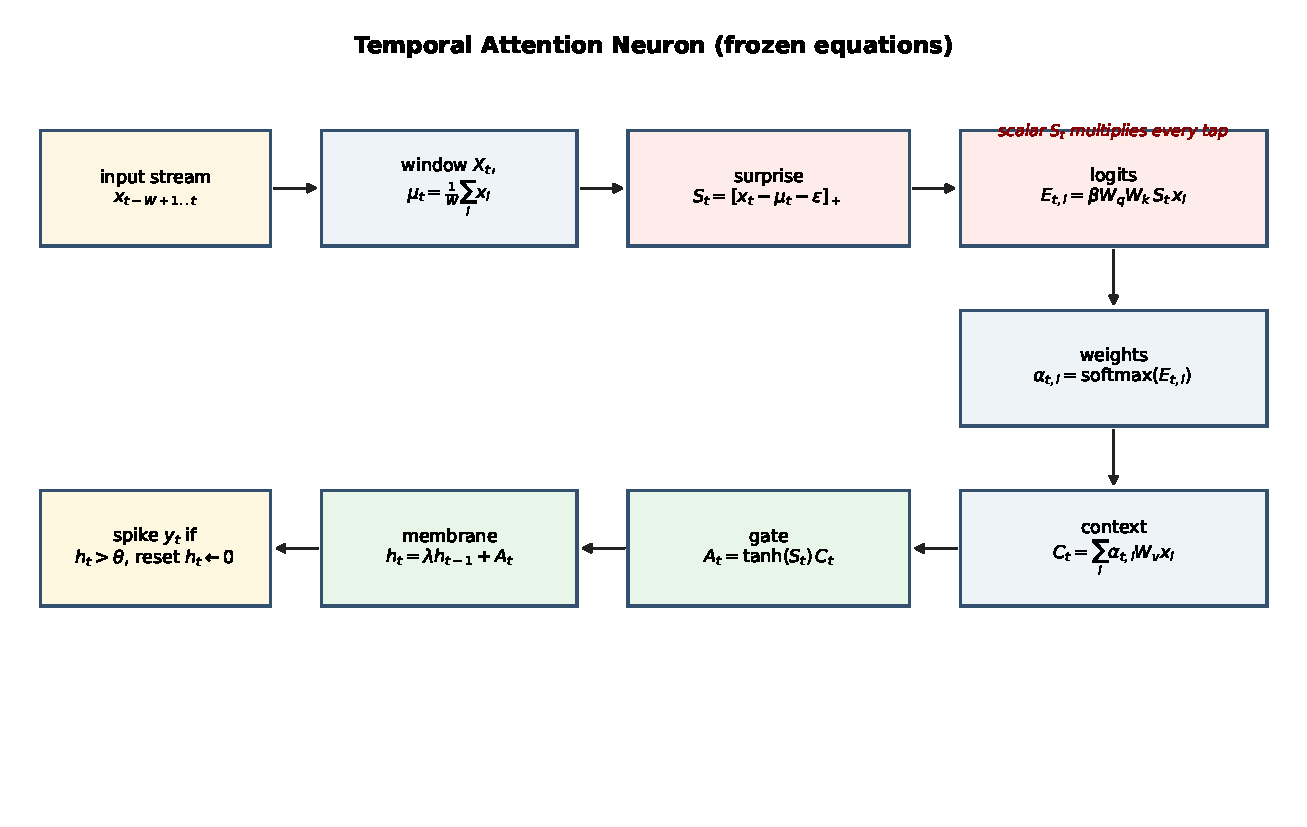
\includegraphics[width=0.78\textwidth]{fig1_architecture.pdf}
  \caption{The frozen TAN architecture and information flow.  The window
  $\mathcal{X}_t$ of the last $W=5$ scalar inputs defines the local mean
  $\mu_t$ and the rectified surprise $S_t$; logits
  $E_{t,i}=\beta W_q W_k S_t x_i$ share the scalar multiplier $S_t$;
  softmax weights $\alpha$ form the context $C_t$; the gate
  $A_t=\tanh(S_t)C_t$ drives the membrane, with spike/\allowbreak{}reset readout.
  Schematic; no data.}
  \label{fig:architecture}
\end{figure}

\begin{figure}[t]
  \centering
  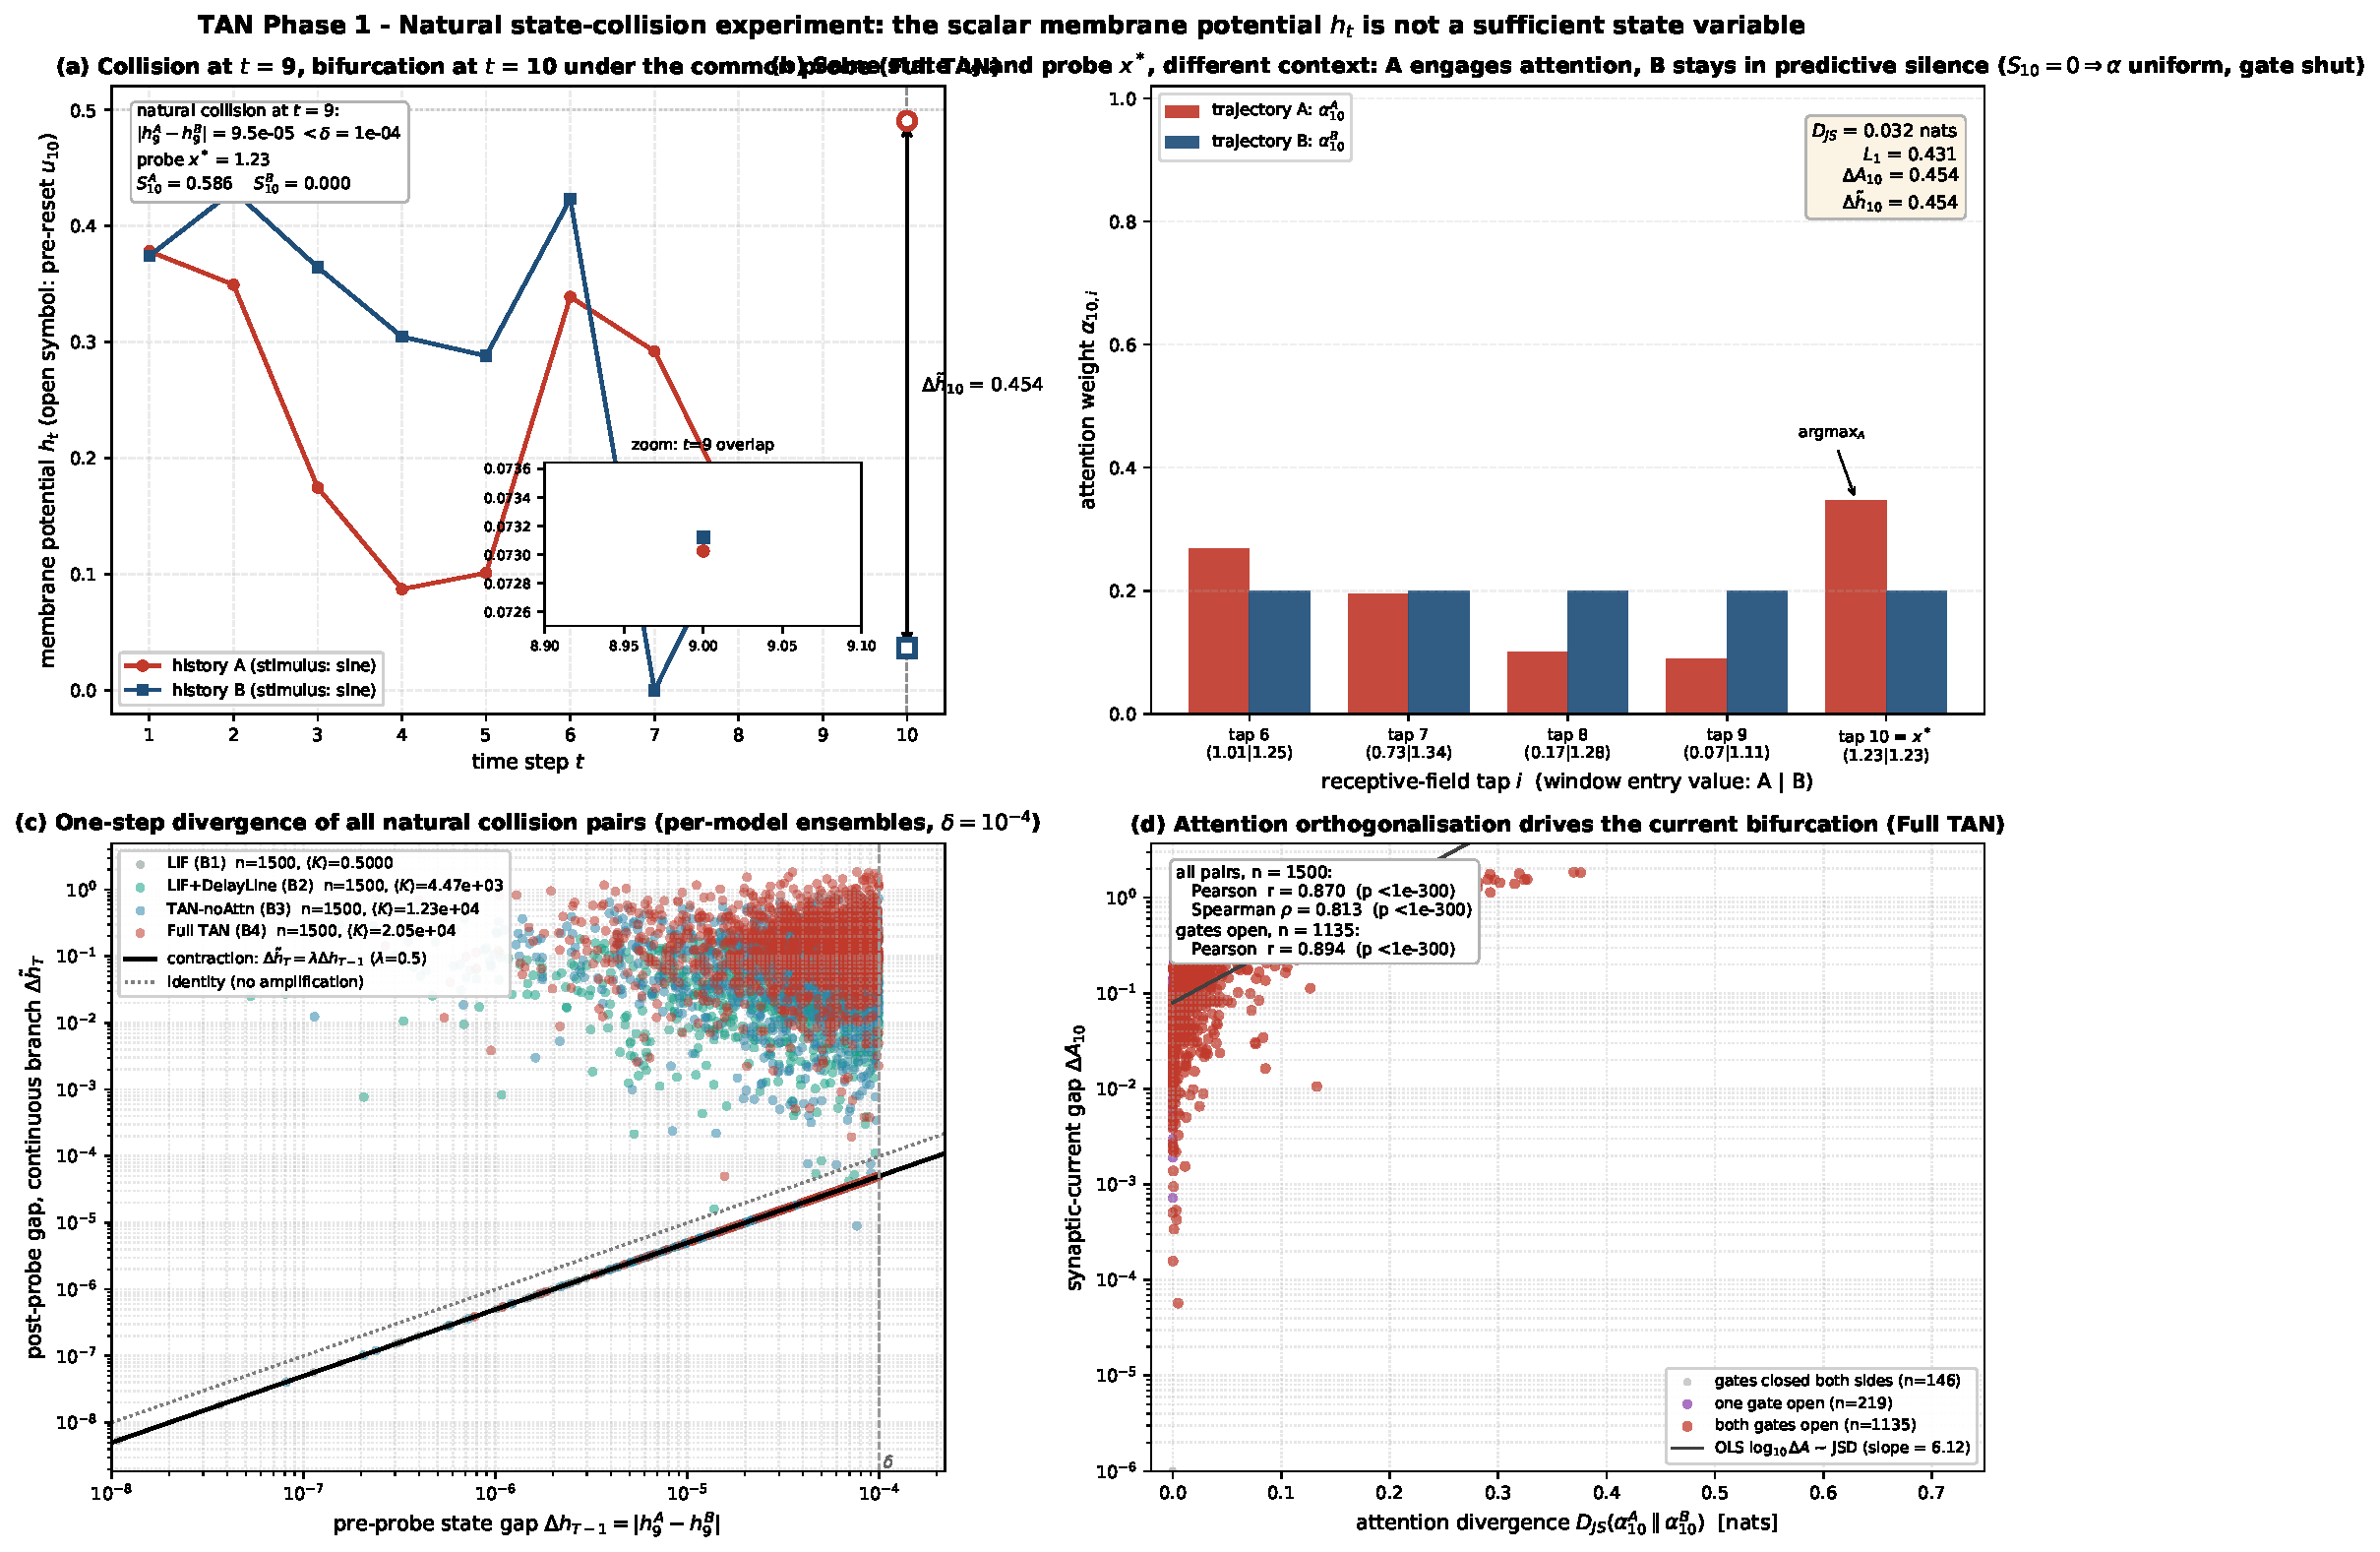
\includegraphics[width=0.95\textwidth]{fig2_state_sufficiency.pdf}
  \caption{Phase 1, natural state collisions (frozen experiment figure
  \texttt{fig22\_\allowbreak{}natural\_\allowbreak{}collision.pdf}, four panels).  (a) A
  representative collision pair: membrane potentials meet within
  $\delta=10^{-4}$ at $t=9$ and bifurcate at the identical probe $t=10$
  (continuous branch); (b) history-conditional attention and gate at the
  probe; (c) one-step divergence $K$ of all collision pairs on log--log
  axes for B1--B4 (B1 lies exactly on the contraction line
  $\Delta\tilde h_T = \lambda \Delta h_{T-1}$); (d) attention divergence
  (Jensen--Shannon) vs.\ synaptic-current gap.  Full statistics in
  Table~\ref{tab:phase1} and the archive report.}
  \label{fig:phase1}
\end{figure}

\begin{figure}[t]
  \centering
  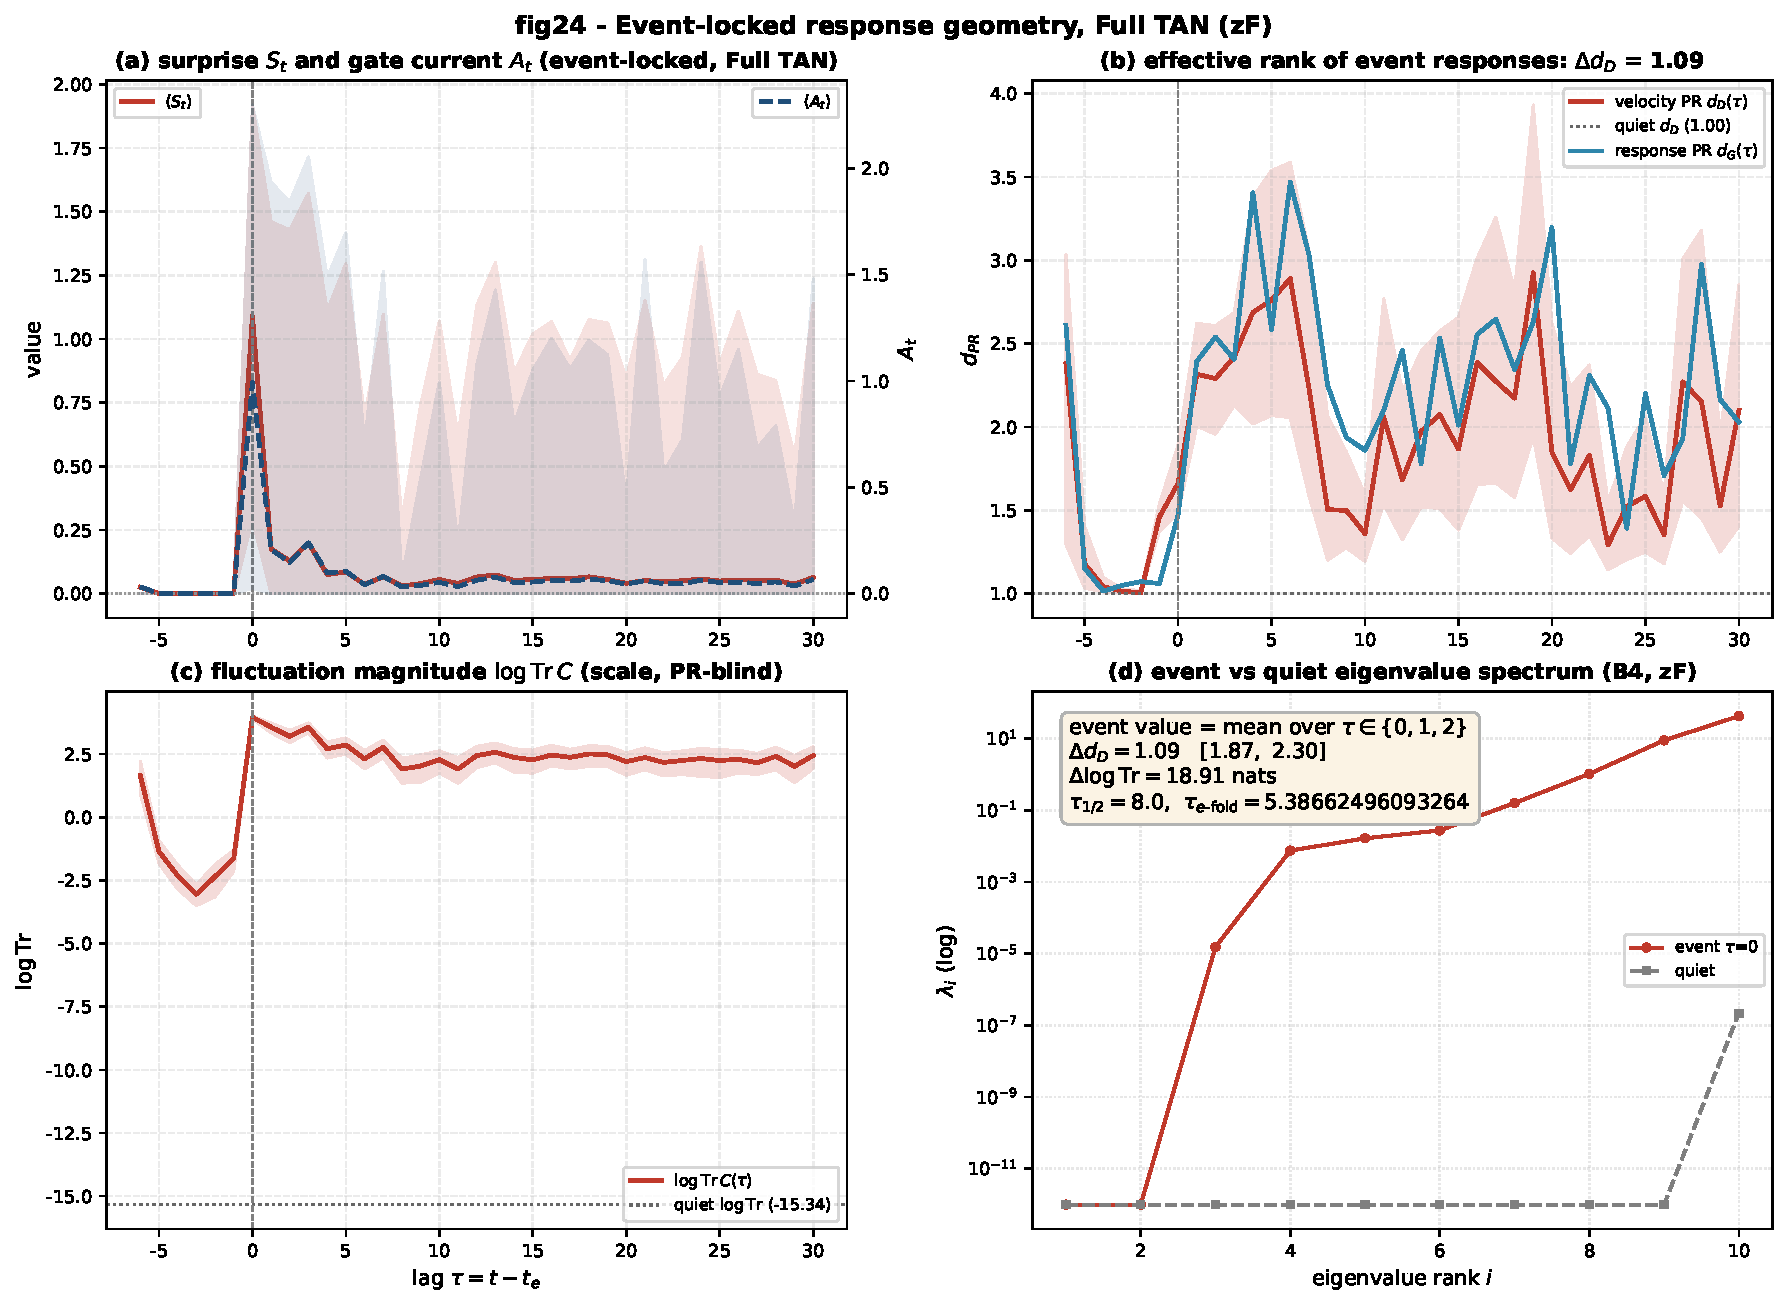
\includegraphics[width=0.95\textwidth]{fig3_geometry.pdf}
  \caption{Phase 2, event-locked geometry of Full TAN in the full frame
  $z_F$ (frozen experiment figure \texttt{fig24\_\allowbreak{}eventlocked.pdf}, four
  panels): (a) event-locked surprise $S_t$ and gated current $A_t$; (b)
  response effective rank $d_G(\tau)$ and velocity rank $d_D(\tau)$ with
  quiet reference; (c) fluctuation scale
  $\log\operatorname{Tr}\,C(\tau)$; (d) event ($\tau=0$) vs.\ quiet
  eigenvalue spectrum.  Effective rank is a covariance statistic, not an
  intrinsic dimension.}
  \label{fig:geometry}
\end{figure}

\begin{figure}[t]
  \centering
  \begin{subfigure}{0.49\textwidth}
    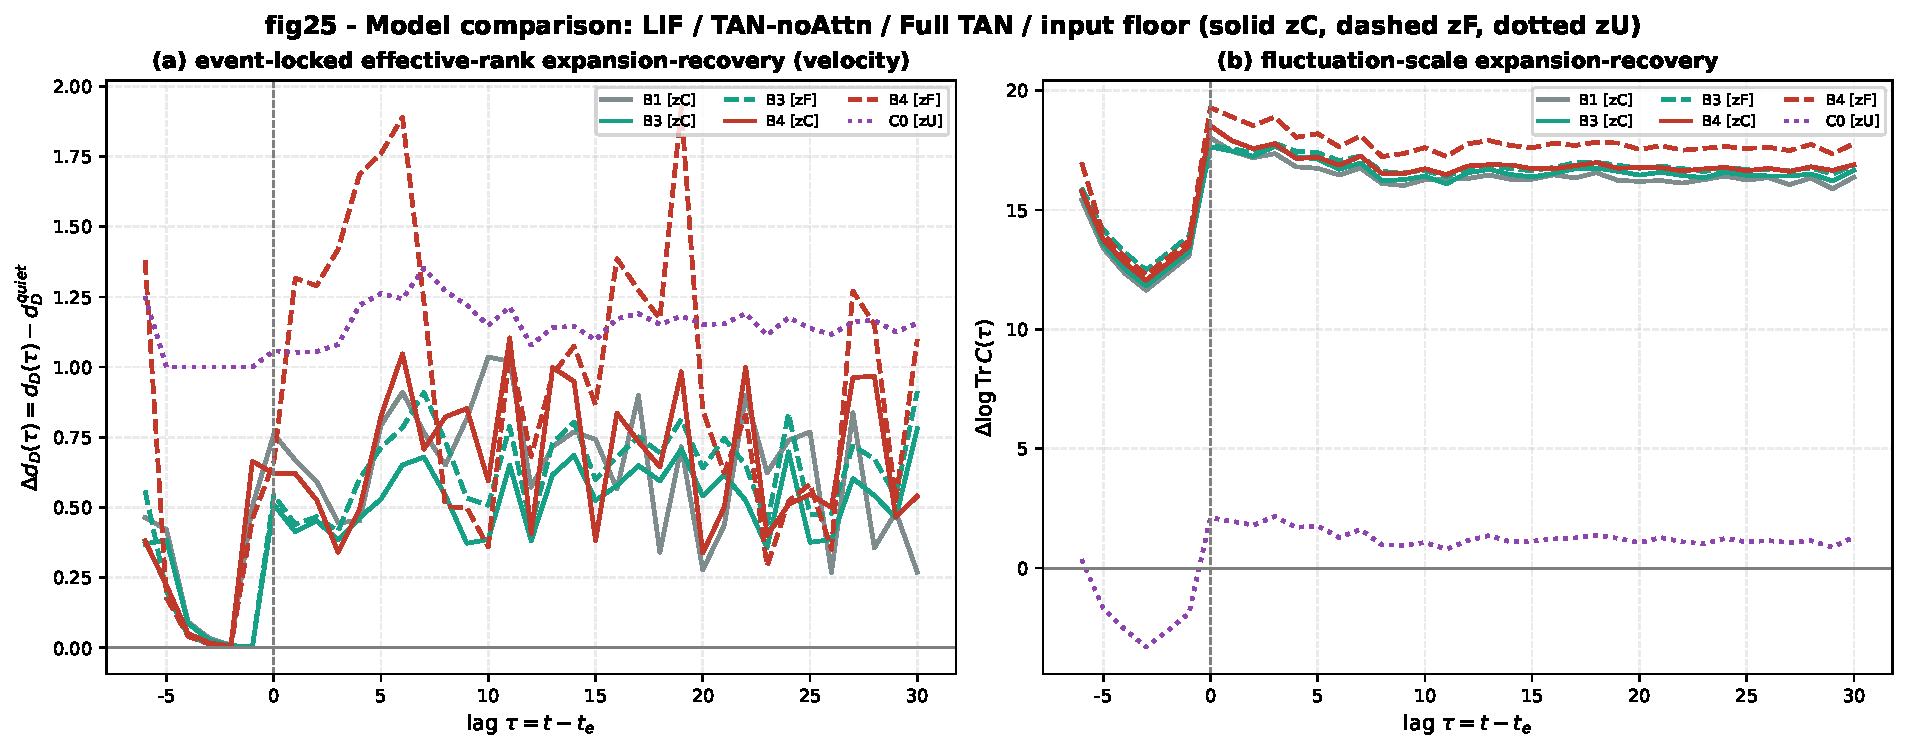
\includegraphics[width=\textwidth]{fig4a_rank_recovery.pdf}
    \caption{Expansion--recovery profiles $\Delta d_D(\tau)$ and
    $\Delta\log\operatorname{Tr}(\tau)$ for B1--B4 and the input control
    (frozen \texttt{fig25\_\allowbreak{}recovery.pdf}; frames: solid $z_C$, dashed
    $z_F$, dotted $z_U$).}
  \end{subfigure}\hfill
  \begin{subfigure}{0.49\textwidth}
    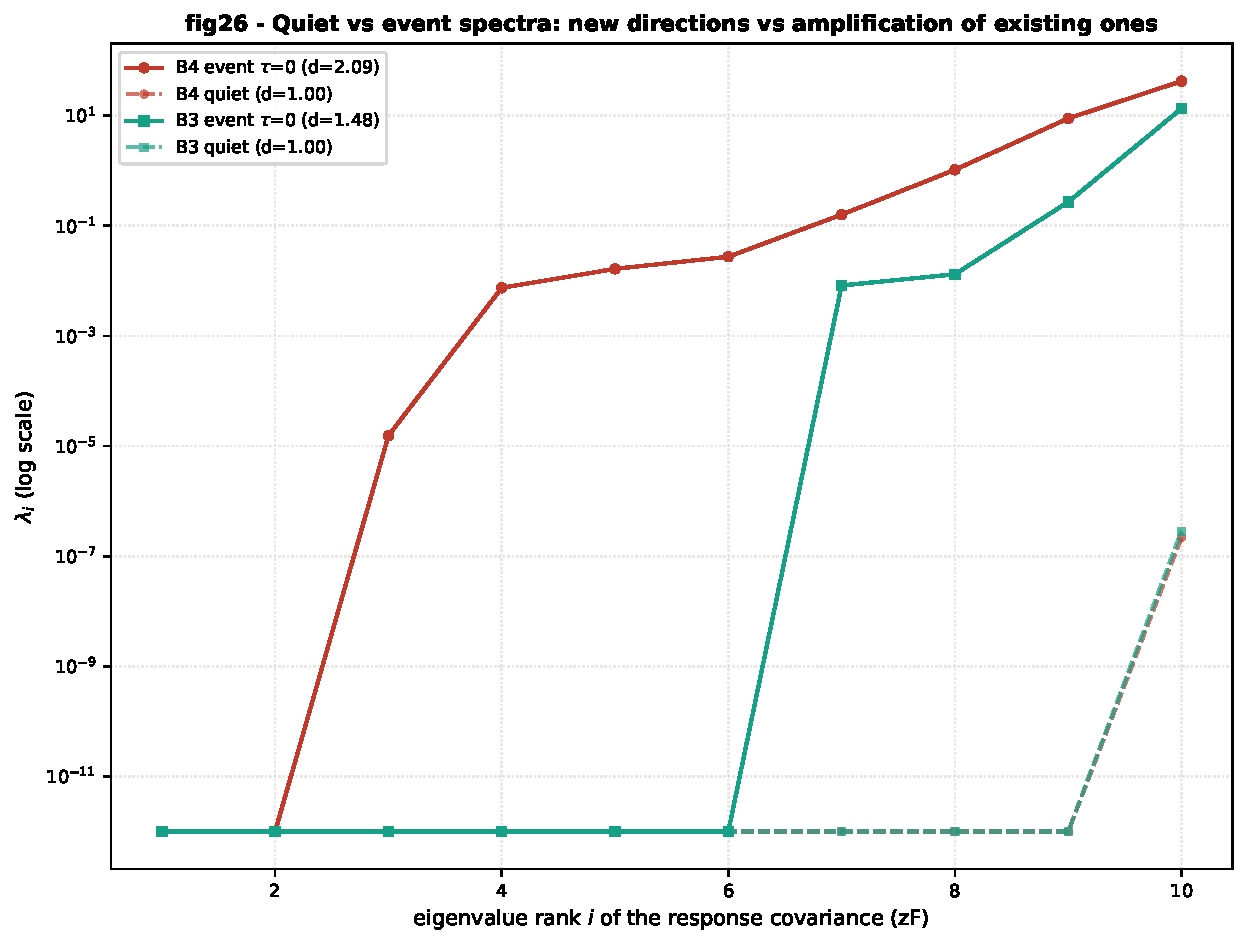
\includegraphics[width=\textwidth]{fig4b_spectra.pdf}
    \caption{Quiet vs.\ event eigenvalue spectra for B4 and B3 in $z_F$
    (frozen \texttt{fig26\_\allowbreak{}spectra.pdf}).  Event-locked expansion adds
    and amplifies directions within the response covariance; see
    Table~\ref{tab:phase2}.}
  \end{subfigure}
  \caption{Phase 2, model comparison in effective rank and scale.  B4
  exceeds B3 in the matched full frame $z_F$ with disjoint event
  confidence intervals and amplitude-control-robust contrasts; in the
  shared frame $z_C$ B4 does not exceed B1.}
  \label{fig:rank}
\end{figure}

\begin{figure}[t]
  \centering
  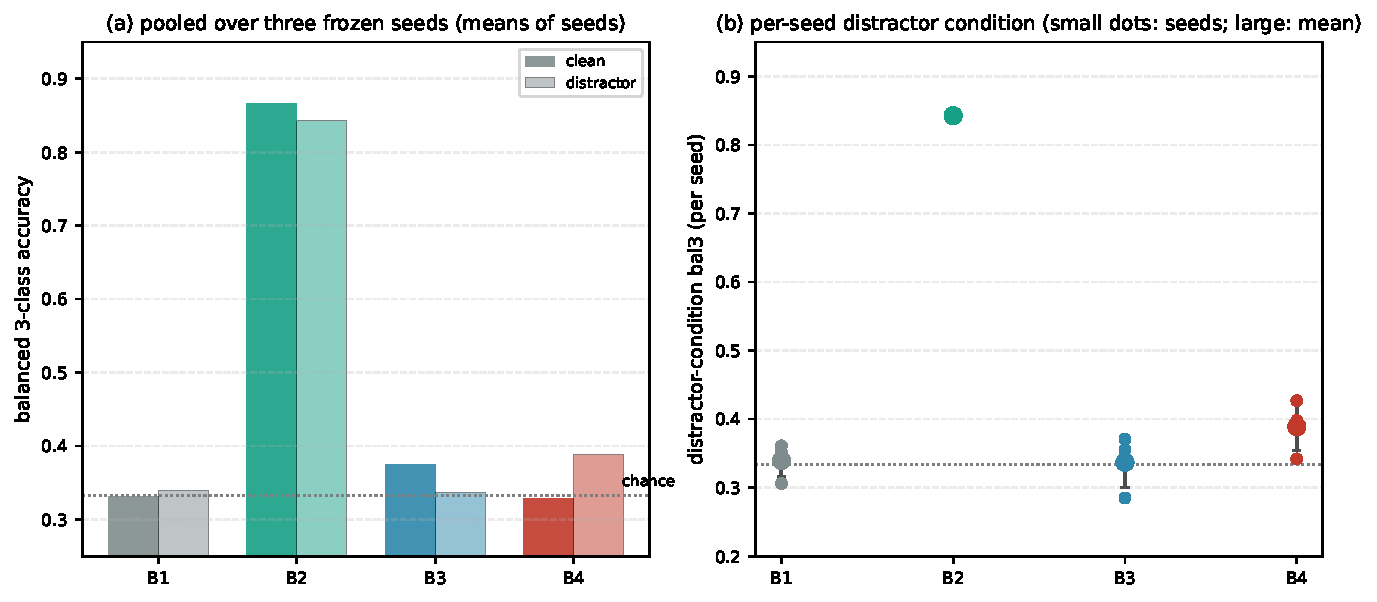
\includegraphics[width=0.92\textwidth]{fig5_probe1.pdf}
  \caption{Probe 1 (frozen three-seed data; values from the amended
  audit documents \texttt{audit\_\allowbreak{}v3\_\allowbreak{}amended/POOLED\_\allowbreak{}PROBE1\_\allowbreak{}V3.md} and
  \texttt{audit\_\allowbreak{}v3\_\allowbreak{}amended/PER\_\allowbreak{}SEED\_\allowbreak{}AUDIT.md}): (a) pooled balanced
  three-class accuracy, clean vs.\ distractor conditions, means over
  three seeds; (b) per-seed distractor-condition accuracy (dots: seeds;
  large dot: mean).  B2 is the strongest fixed-position memory baseline;
  B4 exceeds B3 in the distractor condition (pooled $+0.0570$, 95\% CI
  $[+0.0387,+0.0758]$) with seed-attenuated absolute elevation; B3 has
  lo-blind cells (one invalid for interpretation).}
  \label{fig:probe1}
\end{figure}

\begin{figure}[t]
  \centering
  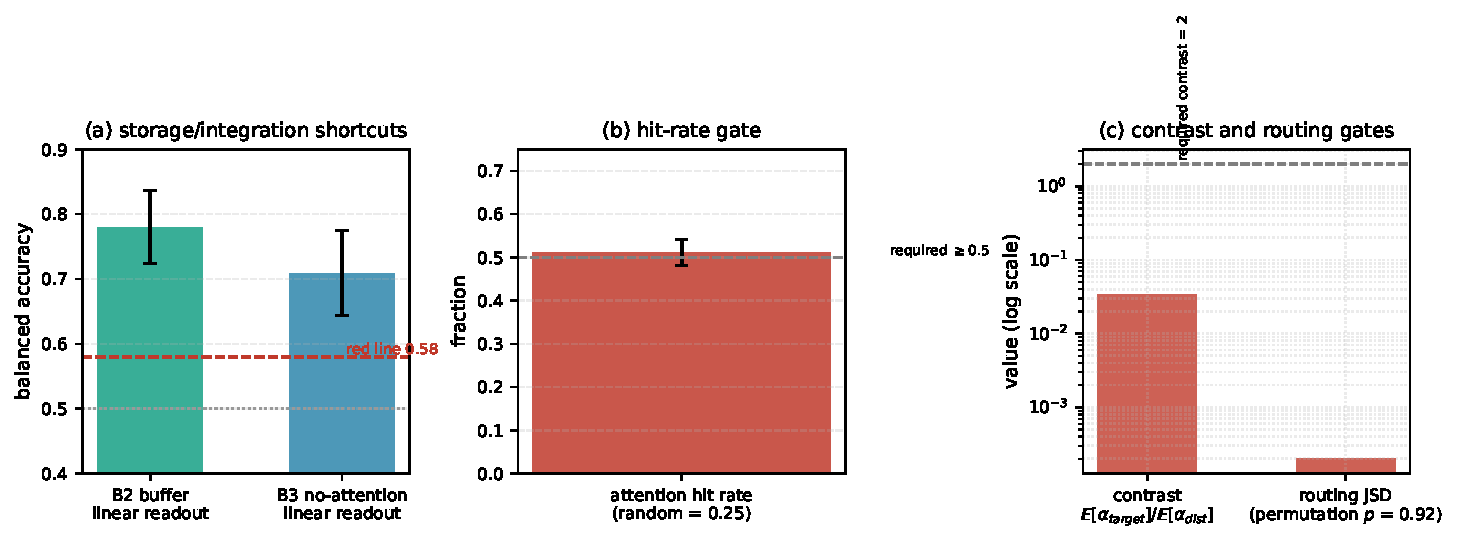
\includegraphics[width=0.96\textwidth]{fig6_probe2.pdf}
  \caption{Probe 2 identifiability audit (values from the frozen audit
  documents \texttt{AUDIT\_\allowbreak{}REPORT.md} / \texttt{AUDIT\_\allowbreak{}OUTPUT.txt}):
  (a) linear-readout shortcuts of B2 (0.779) and B3 (0.709) against the
  0.58 red line; (b) B4 attention hit rate 0.511 (CI
  $[0.481,0.542]$; split $q{=}A$: 0.000, $q{=}B$: 1.000) against the
  0.50 requirement; (c) target/\allowbreak{}distractor contrast $R=0.034$ (required
  $\geq 2$) and query-conditioned JSD $0.0002$ (permutation $p=0.92$).
  Audit status: TERMINATED / AUDIT\_\allowbreak{}FAILED (identifiability boundary).}
  \label{fig:probe2}
\end{figure}

\begin{figure}[t]
  \centering
  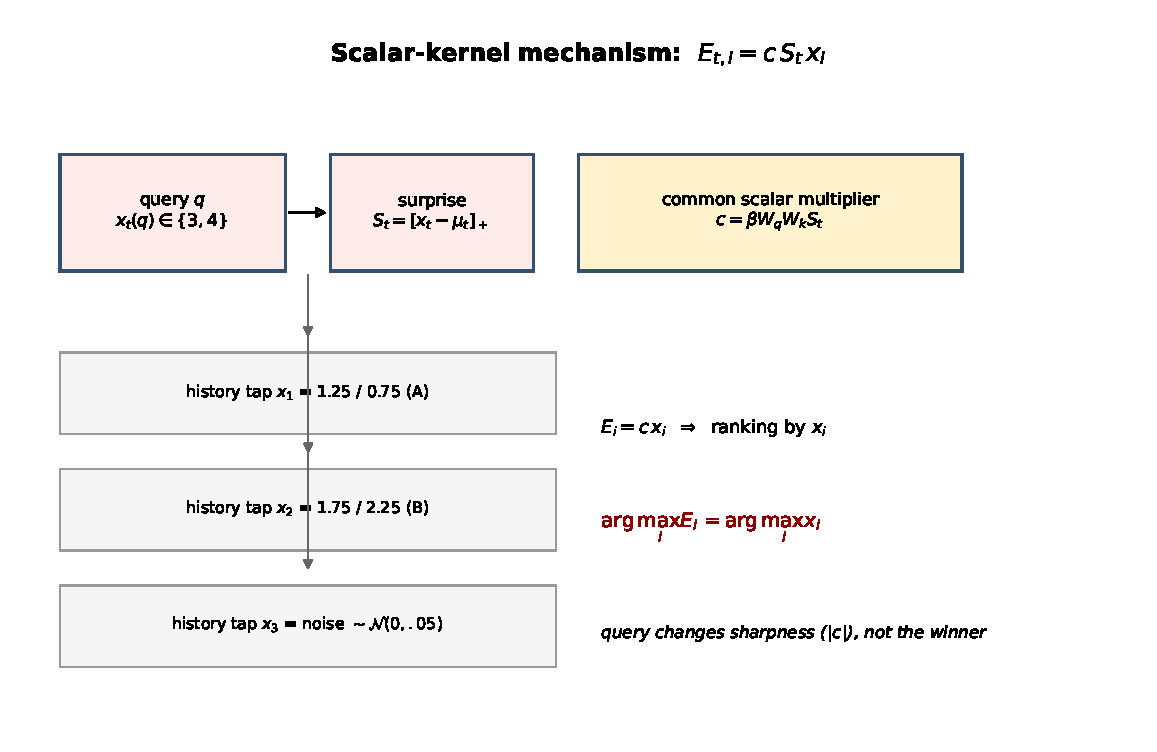
\includegraphics[width=0.82\textwidth]{fig7_mechanism.pdf}
  \caption{Scalar-kernel mechanism: with $E_{t,i}=\gamma_t x_i$ the
  query enters only through the common scalar $\gamma_t \propto S_t$, so
  $\arg\max_i E_{t,i}=\arg\max_i x_i$: the query changes attention
  sharpness, never the winner among history taps.  Schematic; no data.}
  \label{fig:mechanism}
\end{figure}

\begin{figure}[t]
  \centering
  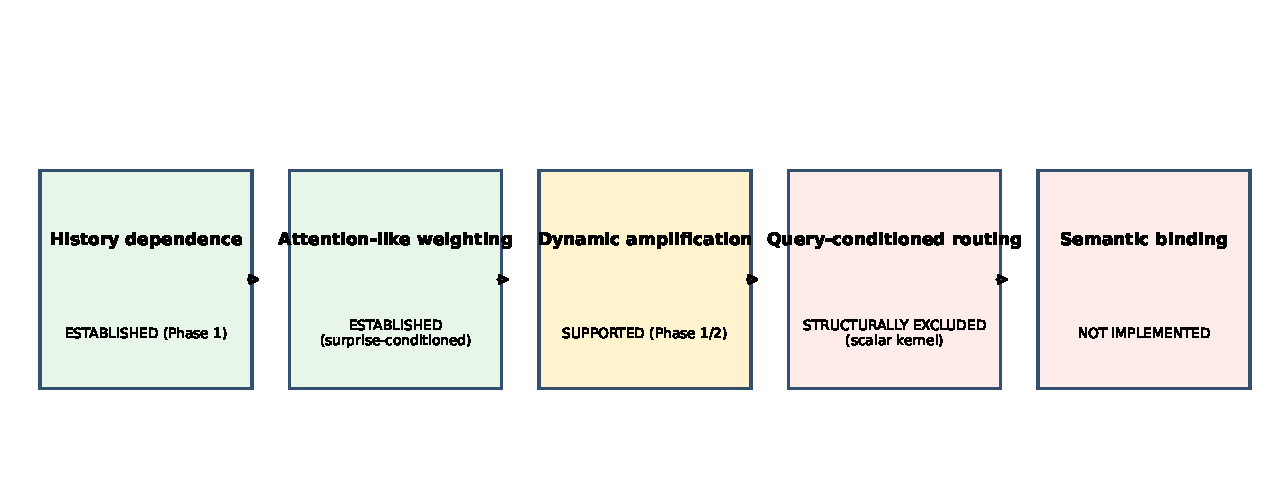
\includegraphics[width=0.95\textwidth]{fig8_summary.pdf}
  \caption{Mechanistic decomposition established by the frozen
  experiments: history dependence and surprise-conditioned weighting are
  established; dynamic amplification is supported; query-conditioned
  routing is structurally excluded by the scalar kernel; semantic
  binding is not implemented.  Schematic; no data.}
  \label{fig:summary}
\end{figure}

% ---------------- tables ----------------
\begin{table}[t]
  \centering
  \caption{Frozen TAN parameters (Section~\ref{sec:model-def}).}
  \begingroup\setlength{\tabcolsep}{8pt}\small\begin{tabular}{@{}llcl@{}}
\toprule
parameter & value & symbol & note \\
\midrule
window length & 5 & $W$ & receptive field \\
leak & 0.5 & $\lambda$ & membrane decay \\
threshold & 0.5 & $\theta$ & spike threshold \\
query weight & 2.0 & $W_q$ & linear map \\
key weight & 1.0 & $W_k$ & linear map \\
value weight & 1.0 & $W_v$ & linear map \\
inverse temperature & 1.0 & $\beta$ & softmax \\
noise tolerance & 0.0 & $\varepsilon$ & dead zone \\
softmax offset & $10^{-9}$ & --- & denominator \\
reset rule & $h_t\!\leftarrow\!0$ & --- & after spike \\
\bottomrule
\end{tabular}\endgroup

  \label{tab:params}
\end{table}

\begin{table}[t]
  \centering
  \caption{Phase 1: one-step continuous-branch amplification $K$ on
  natural collision pairs (1{,}500 per model).  B1 is exactly
  contracting ($K=\lambda=0.5$, max deviation $1.8\times10^{-8}$);
  post-reset Markov violation rate is 0\%, 0.6\%, 33.1\%, 32.2\% for
  B1--B4.  Source: \texttt{natural\_\allowbreak{}collision\_\allowbreak{}summary.csv} (frozen).}
  \begingroup\setlength{\tabcolsep}{3pt}\begin{tabular}{lcccccc}
\toprule
Model & $n$ pairs & mean $K$ & 95\% CI & median $K$ & \% $K{>}10^3$ & post-reset viol. \% \\
\midrule
B1 LIF & 1500 & 5.000e-01 & [5.00e-01, 5.00e-01] & 5.00e-01 & 0.0 & 0.0 \\
B2 LIF+delay & 1500 & 4.470e+03 & [3.26e+03, 5.92e+03] & 8.96e+02 & 46.7 & 0.6 \\
B3 TAN-noAttn & 1500 & 1.235e+04 & [7.78e+03, 1.83e+04] & 1.37e+03 & 56.7 & 33.1 \\
B4 Full TAN & 1500 & 2.047e+04 & [1.12e+04, 3.57e+04] & 2.95e+03 & 73.7 & 32.2 \\
\bottomrule
\end{tabular}\endgroup

  \label{tab:phase1}
\end{table}

\begin{table}[t]
  \centering
  \caption{Phase 2: event velocity effective rank $d_D$ (mean over
  $\tau\in\{0,1,2\}$, 374 pooled events), raw/\allowbreak{}stratified/\allowbreak{}residualised
  amplitude controls, event log-trace, and recovery times.  Sources:
  \texttt{effective\_\allowbreak{}dimension\_\allowbreak{}summary.csv} and
  \texttt{effective\_\allowbreak{}dimension\_\allowbreak{}velocity\_\allowbreak{}eventvalues.csv} (frozen).
  The C0 quiet reference is NaN by policy (zero variance).}
  \begingroup\setlength{\tabcolsep}{5pt}\small\begin{tabular}{@{}cccccccc@{}}
\toprule
Model & frame & $d_D^{ev}$ & $\Delta d_D$ & raw/strat/resid & logTr & $\tau_{e}$ & $\tau_{1/2}$ \\
\midrule
B1 & zC & 1.674 & 0.674 & 1.674/1.732/1.747 & 2.66 & 6.4 & 4 \\
B3 & zC & 1.458 & 0.458 & 1.458/1.495/1.490 & 2.38 & 7.9 & 8 \\
B3 & zF & 1.484 & 0.484 & 1.484/1.509/1.498 & 2.48 & 8.5 & 3 \\
B4 & zC & 1.589 & 0.589 & 1.589/1.701/1.712 & 2.67 & 6.3 & 2 \\
B4 & zF & 2.089 & 1.089 & 2.089/2.250/2.280 & 3.58 & 5.4 & 8 \\
C0 & zU & 1.055 & -- & 1.055/1.051/1.045 & 1.96 & -- & -- \\
\bottomrule
\end{tabular}\endgroup

  \label{tab:phase2}
\end{table}

\begin{table}[t]
  \centering
  \caption{Probe 1 v3: per-seed balanced three-class accuracy with
  amended-audit statuses (24 cells; source:
  \texttt{audit\_\allowbreak{}v3\_\allowbreak{}amended/PER\_\allowbreak{}SEED\_\allowbreak{}AUDIT.md}, frozen).  B3
  20260906 clean $= 0.470$ is marked INVALID\_\allowbreak{}FOR\_\allowbreak{}INTERPRETATION
  (lo-blind); at-chance collapsed cells are PASS\_\allowbreak{}WITH\_\allowbreak{}FLAG.}
  \begingroup\setlength{\tabcolsep}{3pt}\small\begin{tabular}{@{}lllcp{3.15cm}p{3.15cm}@{}}
\toprule
seed & model & condition & bal3 & coverage status & final status \\
\midrule
20260904 & B1 & clean & 0.346 & PASS\_\allowbreak{}WITH\_\allowbreak{}FLAG & PASS\_\allowbreak{}WITH\_\allowbreak{}FLAG \\
20260904 & B1 & dist & 0.352 & PASS\_\allowbreak{}WITH\_\allowbreak{}FLAG & PASS\_\allowbreak{}WITH\_\allowbreak{}FLAG \\
20260904 & B2 & clean & 0.868 & PASS & PASS \\
20260904 & B2 & dist & 0.847 & PASS & PASS \\
20260904 & B3 & clean & 0.333 & PASS\_\allowbreak{}WITH\_\allowbreak{}FLAG & PASS\_\allowbreak{}WITH\_\allowbreak{}FLAG \\
20260904 & B3 & dist & 0.371 & PASS\_\allowbreak{}WITH\_\allowbreak{}FLAG & PASS\_\allowbreak{}WITH\_\allowbreak{}FLAG \\
20260904 & B4 & clean & 0.328 & PASS & PASS \\
20260904 & B4 & dist & 0.427 & PASS & PASS \\
20260905 & B1 & clean & 0.318 & PASS & PASS \\
20260905 & B1 & dist & 0.306 & PASS & PASS \\
20260905 & B2 & clean & 0.857 & PASS & PASS \\
20260905 & B2 & dist & 0.841 & PASS & PASS \\
20260905 & B3 & clean & 0.322 & PASS & PASS \\
20260905 & B3 & dist & 0.355 & PASS & PASS \\
20260905 & B4 & clean & 0.329 & PASS & PASS \\
20260905 & B4 & dist & 0.398 & PASS & PASS \\
20260906 & B1 & clean & 0.329 & PASS\_\allowbreak{}WITH\_\allowbreak{}FLAG & PASS\_\allowbreak{}WITH\_\allowbreak{}FLAG \\
20260906 & B1 & dist & 0.361 & PASS\_\allowbreak{}WITH\_\allowbreak{}FLAG & PASS\_\allowbreak{}WITH\_\allowbreak{}FLAG \\
20260906 & B2 & clean & 0.877 & PASS & PASS \\
20260906 & B2 & dist & 0.840 & PASS & PASS \\
20260906 & B3 & clean & 0.470 & INVALID\_\allowbreak{}FOR\_\allowbreak{}INTER\allowbreak{}PRETATION & INVALID\_\allowbreak{}FOR\_\allowbreak{}INTER\allowbreak{}PRETATION \\
20260906 & B3 & dist & 0.285 & PASS & PASS \\
20260906 & B4 & clean & 0.329 & PASS & PASS \\
20260906 & B4 & dist & 0.342 & PASS & PASS \\
\bottomrule
\end{tabular}\endgroup

  \label{tab:probe1}
\end{table}

\begin{table}[t]
  \centering
  \caption{Probe 2 identifiability audit summary (frozen).  Status:
  TERMINATED / AUDIT\_\allowbreak{}FAILED: a mechanistic identifiability boundary,
  not an incomplete experiment.}
  \begingroup\setlength{\tabcolsep}{3pt}\begin{tabular}{p{4.7cm}p{5.3cm}p{4.9cm}}
\toprule
audit & measured & requirement / gate \\
\midrule
B2 linear readout BA & 0.779 [0.724, 0.836] & $\leq 0.58$ (FAIL) \\
B3 linear readout BA & 0.709 [0.644, 0.775] & $\leq 0.58$ (FAIL) \\
attention hit rate & 0.511 [0.481, 0.542] & $\geq 0.50$ (FAIL); $q{=}A$: 0.000, $q{=}B$: 1.000 \\
target/distractor contrast $R$ & 0.034 & $\geq 2.0$ (FAIL) \\
query-conditioned JSD & 0.0002 & permutation $p{=}0.92$ (FAIL) \\
counterfactual argmax flip & 0.000 & $>0$ required (FAIL) \\
single-tap conditional bias & up to 0.45--0.60 at B-codes & structural note \\
\bottomrule
\end{tabular}\endgroup

  \label{tab:probe2}
\end{table}

\begin{table}[t]
  \centering
  \caption{Claim ledger of this paper (evidence levels follow the frozen
  archive claim ledger, \texttt{docs/CLAIM\_\allowbreak{}LEDGER.md}).}
  \begingroup\setlength{\tabcolsep}{3pt}\begin{tabular}{p{7.7cm}p{4.3cm}p{2.5cm}}
\toprule
claim & status & evidence \\
\midrule
$h_t$ is a sufficient Markov state & REJECTED & Phase 1 \\
TAN is history-dependent & ESTABLISHED & Phase 1 \\
higher intrinsic dimension than LIF & NOT SUPPORTED & Phase 2 \\
event-locked geometry reorganises (rank/scale) & SUPPORTED & Phase 2 \\
fixed buffer can outperform TAN & ESTABLISHED & Probe 1 \\
improved retrieval in content-rich context (vs no-attn) & LIMITED SUPPORT & Probe 1 \\
distractor robustness & NOT ESTABLISHED & Probe 1 \\
genuine Q--K routing / query-conditioned selection & REJECTED / STRUCTURALLY EXCLUDED & Probe 2 + theory \\
surprise-conditioned saliency weighting & ESTABLISHED & theory + all phases \\
\bottomrule
\end{tabular}\endgroup

  \label{tab:claims}
\end{table}

\newpage
\section*{Data and Code Availability}
The frozen research archive accompanying this paper contains all
experiment scripts, seeds, logs, tables, figures and audit documents:
Phase 1 (\texttt{code/experiments/natural\_\allowbreak{}collision.py}), Phase 2
(\texttt{code/experiments/effective\_\allowbreak{}dimension.py}), Probe 1
(\texttt{code/experiments/temporal\_\allowbreak{}distractor.py}), Probe 2
(\texttt{code/\allowbreak{}experiments/\allowbreak{}probe2/\allowbreak{}identifiability/\allowbreak{}}), model reference
(\texttt{code/\allowbreak{}model/\allowbreak{}tan.py}), archive index
(\texttt{code/RESEARCH\_\allowbreak{}ARCHIVE\_\allowbreak{}INDEX.md}) and reproducibility ledger
(\texttt{docs/REPRODUCIBILITY\_\allowbreak{}LEDGER.md}).  Figures~2--6 reproduce
frozen experiment figures or are drawn from frozen result documents; no
new experiment was performed for this paper.

\section*{Reproducibility Statement}
All experiments use deterministic seeds and frozen parameters; audit
statuses (including Probe 2 = TERMINATED / AUDIT\_\allowbreak{}FAILED) are archived;
no post-hoc tuning was performed; per-seed tables and the archive
integrity statement are provided (\texttt{audit\_\allowbreak{}v3\_\allowbreak{}amended/},
\texttt{docs/\allowbreak{}}).  The PDF is built with the command in
\texttt{paper/\allowbreak{}Makefile} (equivalently: \texttt{pdflatex main.tex;
bibtex main; pdflatex main.tex; pdflatex main.tex}).

\section*{Conflict of Interest}
The author declares no competing interests.

\section*{Acknowledgements}
The author thanks the reviewers of the archived research programme for
insisting on identifiability audits and on the separation of claims
documented in this paper.

\bibliographystyle{plainnat}
\bibliography{references}

% ---------------- supplementary ----------------
\appendix
% S1: detailed equations
\section{Supplementary S1: Detailed TAN equations and conventions}

The frozen model used in every experiment of this paper:

\begin{align}
  \mathcal{X}_t &= [x_{t-W+1},\dots,x_t], & W &= 5,\\
  \mu_t &= \tfrac1W \textstyle\sum_i x_{t-W+i}, & x_t &\in \mathbb{R},\\
  S_t &= [x_t - \mu_t - \varepsilon]_+, & \varepsilon &= 0,\\
  Q_t &= W_q S_t,\quad K_{t,i}=W_k x_{t-W+i},\quad V_{t,i}=W_v x_{t-W+i},
    & W_q&=2.0,\; W_k=W_v=1.0,\\
  E_{t,i} &= Q_t K_{t,i}, & &\\
  \alpha_{t,i} &= \frac{\exp(\beta E_{t,i})}{\sum_{j=1}^W
    \exp(\beta E_{t,j}) + 10^{-9}}, & \beta &= 1.0,\\
  C_t &= \textstyle\sum_i \alpha_{t,i} V_{t,i}, & &\\
  A_t &= \tanh(S_t)\,C_t, & &\\
  h_t &= \lambda h_{t-1} + A_t, & \lambda &= 0.5,\\
  y_t &= \mathbb{1}[h_t > \theta],\quad h_t \leftarrow 0 \text{ if }
    y_t = 1, & \theta &= 0.5 .
\end{align}

Conventions: the window includes the current input $x_t$; the receptive
field is zero-padded at trial onset (stimulus onset after silence); the
initial membrane potential is $h_0 = 0$; surprise is computed with
$\mu_t$ over the window including $x_t$; a spike occurs when the
pre-reset potential exceeds $\theta$ strictly, followed by reset.  The
vectorised experiment implementations were parity-checked against the
scalar reference implementation \texttt{code/model/tan.py} (worst deviation in
$h$: $1.5\times10^{-10}$; spike agreement exact).

% S2
\section{Supplementary S2: Phase 1 collision analysis details}

\textbf{Stimulus pool.} $N = 160{,}000$ histories of length $T-1 = 9$
($4\times40{,}000$ per stimulus family: Gaussian white noise, random
step, ramp, sine), seed 20260726.

\textbf{Collision ensembles (per model).} Pairs with both potentials in
the subthreshold band $(0.05,\theta)$ at $t=9$ and
$|h_9^A - h_9^B| < \delta = 10^{-4}$: B1 92{,}600 pairs, B2 19{,}234,
B3 1{,}633{,}844, B4 1{,}427{,}817; 1{,}500 analysed per model.  The
band excludes reset-induced $h=0$ coincidences by construction.

\textbf{One-step probe.} An identical probe
$x^*\sim\mathcal{U}(0.5,3.0)$ was injected at $t=10$; divergence was
measured on the continuous branch ($u_{10} = \lambda h_9 + A_{10}$)
because the threshold/reset is a readout discontinuity shared by all
four models.  Post-reset divergence and spike-outcome classes are
tabulated separately.

\textbf{Key statistics (frozen).} Mean $K$: B1 $0.5000000$ (exact),
B2 $4.47\times10^3$ [$3.26,5.92$], B3 $1.235\times10^4$
[$7.78,1.83$], B4 $2.047\times10^4$ [$1.12,3.57$] (95\% bootstrap).
$K>10^3$ in 0/46.7/56.7/73.7\% of pairs.  Gate-closed collisions
($S_{10}=0$, both sides): $K = 0.5$ exactly.  Probe outcomes
(none/one/both spiked): B1 0/0/100\%; B2 0.1/0.5/99.4\%; B3
38.9/7.1/54.1\%; B4 33.3/8.6/58.1\%; post-reset violations 0/0.6/33.1/
32.2\%.  Correlations (B4): Pearson $r(\mathrm{JSD},\Delta A)=0.870$
(all pairs) and 0.894 (both gates open), $p<10^{-300}$;
$r(\Delta A,\Delta\tilde h)=1.000$.  Cross-model log-$K$ comparisons:
B4 vs.\ B3 $p=1.3\times10^{-32}$ (median ratio 2.15), B4 vs.\ B2
$p=1.3\times10^{-63}$ (3.29), B2 vs.\ B1 $p<10^{-300}$.

\textbf{Reset re-bifurcation.} $n=843$ pairs in which all four models
double-spike at $t=10$ (identical observable state $h_{10}=0$) continue
with identical inputs: B1 gap $\equiv 0$ (machine-exact); B2 re-diverges
on the continuous branch ($\langle|\Delta u|\rangle = 0.115$ at
$t=11$) and returns to zero after the window flush ($t=14$); B3/B4
re-divergence decays but $\sim$25\% of pairs retain gaps $>10^{-3}$ at
$t=18$.

\textbf{Interpretation.} The projection $\pi:(h,\bar X)\mapsto h$ is not
lumpable: on surprise-open fibres the next-state map is context-valued.
History dependence is shared by all window-carrying models (B2, B3, B4);
attention modulates its magnitude and the gate makes it conditional on
prediction error.

% S3
\section{Supplementary S3: Phase 2 methodology}

\textbf{Observables and frames.} Response trajectories are embedded as
$z_U = [\mu, S, x]$ (input-only control C0), $z_C = [h,\mu,S,A]$
(models B1--B4; for B1, $A:=x_t$ is a recorded null convention) and
$z_F = [h,\mu,S,A,\alpha_1,\dots,\alpha_5,C]$ (B3/B4 only; for B3,
$\alpha_i \equiv 1/5$ and $C = \mu$ by definition -- a degenerate but
not noise-filled coordinate set).

\textbf{Standardisation and pooling.} Coordinates are globally
$Z$-scored per seed (post-burn-in statistics); coordinates with
$\sigma < 10^{-12}$ are treated as constant and set to zero (counted,
never noise-filled).  No full covariance whitening is applied.  Because
per-seed $Z$-scoring assigns arbitrary per-seed levels, quiet blocks and
the raw-state secondary matrices are centred per seed before cross-seed
pooling; $\Delta z$ and velocity quantities cancel those levels by
construction, so all decision variables are unaffected (estimator note
recorded in the archive log).

\textbf{Event-locked geometry.} Episodes are onset-aligned,
$\tau \in [-6,30]$; only events with a clean five-step pre-window are
kept (374 pooled events across three seeds).  Primary response:
$\Delta z_{e,\tau} = z'_{e,\tau} - \bar z'_{e,\mathrm{pre}}$;
velocity $v_{e,\tau} = z'_{e,\tau+1}-z'_{e,\tau}$ (same-event adjacent
increments).  Effective rank $d = \mathrm{Tr}^2/\mathrm{Tr}^2$ of the
pooled covariance at fixed $\tau$; $\log\mathrm{Tr}$ and eigenvalue
spectra always accompany $d$ (PR is scale-invariant and cannot detect
pure amplification).  NaN policy: $n < 30$ or
$\mathrm{Tr} \le 10^{-12}$ returns NaN (never 1).  Amplitude controls:
raw pooled; median-split stratification with pooled-within covariance;
per-coordinate linear residualisation on $\log_{10}$ amplitude.

\textbf{Quiet reference and recovery.} Quiet samples lie $\geq 12$
steps from any pulse (mutual spacing $\geq 12$).  Recovery is estimated
on isolated events (next onset beyond $\tau = 30$): $\tau_{1/2}$ on
$d_D$ and $\tau_{e\text{-fold}}$ from a linear fit of
$\log\mathrm{Tr}(\tau)$ (requires $\geq 0.3$ nats drop), with event
bootstrap 95\% CIs.

\textbf{Decision gates (pre-registered).} Event value = mean over
$\tau \in \{0,1,2\}$; stable expansion $\Delta d_D \geq 0.5$ with CI
excluding 0.  Outcome A (TAN-specific rank expansion beyond controls)
requires the full-frame B4 $>$ B3 contrast \emph{and} a shared-frame
B4 $>$ B1 contrast; outcome B (scale/amplification channel) requires
$\Delta\log\mathrm{Tr}(\mathrm{B4}) - \Delta\log\mathrm{Tr}(\mathrm{B3})
\geq 0.2$ nats; the archived gate fell to D (by exclusion) because the
shared-frame B4 vs.\ B1 leg failed -- recorded, not retuned.

% S4
\section{Supplementary S4: Probe 1 complete per-seed results}

Probe-1 v3 (frozen): target at step 5 with class
$c_T$ (lo $\sim\mathcal{U}(0.55,1.05)$, hi $\sim\mathcal{U}(0.95,1.45)$),
three distractors (same mixture) or silence, query at step 9 (retrieval
cue, not in the label), catch trials with no target (one third); label
three-way (lo/hi/absent); linear 3-class softmax on the response
trajectory $[u_9..u_{13}, y_9..y_{13}]$; train 4000 / test 2000 per seed;
seeds 20260904/05/06.  The full 24-cell per-seed audit table is in
Table~\ref{tab:probe1} (main text).  Per-seed balanced 3-class accuracy:

\begin{center}
\small
\begin{tabular}{lcccccc}
\toprule
seed & cond. & B1 & B2 & B3 & B4 \\
\midrule
20260904 & clean & 0.346 & 0.868 & 0.333 & 0.328 \\
20260904 & distractor & 0.352 & 0.847 & 0.371 & 0.427 \\
20260905 & clean & 0.318 & 0.857 & 0.322 & 0.329 \\
20260905 & distractor & 0.306 & 0.841 & 0.355 & 0.398 \\
20260906 & clean & 0.329 & 0.877 & 0.470$^{*}$ & 0.329 \\
20260906 & distractor & 0.361 & 0.840 & 0.285 & 0.342 \\
\bottomrule
\end{tabular}
\end{center}

$^{*}$ B3 20260906 clean $= 0.470$ accompanies lo-class blindness in the
readout; this cell is INVALID\_\allowbreak{}FOR\_\allowbreak{}INTERPRETATION (the nominal value is
retained in the archive but is not treated as healthy 3-class decoding).
At-chance cells with collapsed class coverage are flagged
PASS\_\allowbreak{}WITH\_\allowbreak{}FLAG and excluded from claims.  Pooled contrasts (n = 6000
test trials): B4 $-$ B3 distractor $+0.0570$ (95\% CI
$[+0.0387,+0.0758]$); per-seed differences $+0.056/+0.043/+0.056$.  B4
absolute distractor-condition bal3: 0.427 / 0.398 / 0.342 (attenuates;
seed 20260906 $\approx$ chance).  B2 is the strongest model in every
seed (fixed-position memory baseline).  B1 $\approx$ chance.  Shuffled-
label controls return to chance under the amended permutation-null
audit.

% S5
\section{Supplementary S5: Probe 1 amended-audit methodology}

The three-seed Probe-1 run was blocked before pooling by two
pre-registered audit-statistic gates.  Per the frozen-data rule (never
re-run or modify the experiment), the audit statistics were amended and
re-applied to the frozen three-seed data only; no experiment parameter
changed.  The deterministic reproduction of the frozen pipeline was
verified against the frozen per-seed numbers (maximum deviation
$4.7\times10^{-4}$, which equals the 3-decimal rounding of the frozen
table).

\textbf{A1 -- shuffle audit.} The fixed gate on the mean over ten
shuffles of the shuffled-label balanced accuracy (threshold 0.37) was
abolished: L-BFGS on permuted labels
has a heavy-tailed overfit distribution (n=1500: 25-shuffle mean 0.346,
sd 0.079; at n=4000 the mean-of-10 sd is $\approx 0.025$; the offending
B2 seed-3 value 0.378 was $\approx +1.1\sigma$ noise, not leakage).  The
amended audit uses an empirical permutation null (100 label
permutations per seed $\times$ model, refit each time) and classifies
each cell PASS / PASS\_\allowbreak{}WITH\_\allowbreak{}QC\_\allowbreak{}LIMITATION /
INVALID\_\allowbreak{}FOR\_\allowbreak{}INTERPRETATION from the null mean and a z-score.

\textbf{A2 -- class-coverage audit.} A never-predicted class no longer
blocks the run.  At-chance cells with a missing class are
PASS\_\allowbreak{}WITH\_\allowbreak{}FLAG (collapse expected; excluded from claims); above-chance
cells with a missing class ($\geq 20$ true samples) are
INVALID\_\allowbreak{}FOR\_\allowbreak{}INTERPRETATION; a pattern persistent in $\geq 2/3$ seeds
sets a model-level flag.  B3's lo-blindness occurred in 1/3 seeds by the
overall criterion (seed 1 overall; seed 3 clean cell), so no persistent
model-level flag is set; the affected cells carry their own statuses.

\textbf{Statuses.} 24-cell table in Table~\ref{tab:probe1}; all shuffle
statuses PASS; B3 20260906 clean INVALID\_\allowbreak{}FOR\_\allowbreak{}INTERPRETATION; B1
at-chance cells PASS\_\allowbreak{}WITH\_\allowbreak{}FLAG.  Pooling was performed after the
amended table and preserves per-seed detail, the B3 caveat and the B4
seed-3 attenuation.  Machine-readable audit decisions:
(\texttt{audit\_\allowbreak{}v3\_\allowbreak{}amended/MACHINE\_\allowbreak{}READABLE\_\allowbreak{}AUDIT.json}).

% S6
\section{Supplementary S6: Probe 2 full audit results}

Frozen audit (\texttt{probe2\_\allowbreak{}identifiability\_\allowbreak{}audit.py}, seed 20260904,
$N=1000$, $W=5$, $\sigma_{\text{noise}}=0.05$; archive:
\texttt{code/experiments/probe2/identifiability/}).  Status:
\texttt{TERMINATED / AUDIT\_\allowbreak{}FAILED}.

\textbf{Generator.} Position balance over the four slots (A+B counts
506/476/492/526, $\chi^2$ $p=0.44$); query--label mutual information
$I(q;y)\approx 3\times10^{-4}$ ($\chi^2$ $p=0.47$); best single-slot
balanced accuracy $0.555$ [$0.487,0.625$] (below the 0.58 gate).
Structural note: at B-coded amplitude values the conditional expectation
$|\mathbb{E}[V_q \mid x_i]|$ reaches 0.45--0.60 (e.g.\ $x_i = 2.25$
implies $y=+1$ on the $q=B$ half of trials), so the encoding is not
strictly leakage-free by the \texttt{}$\mathbb{E}[V_q|x_i]\approx 0$''
criterion; this is recorded as an encoding-level confound.

\textbf{Audit A (B2 linear readout on $[x_{t-4},\dots,x_t]$).}
Balanced accuracy $0.7789$ [$0.7236,0.8358$] --- FAIL (red line 0.58).
\textbf{Audit B (B3 uniform-integration features).} $0.7094$
[$0.6435,0.7745$] --- FAIL.  Both shortcuts follow from the asymmetric
key amplitudes: the B-coded event is the largest history tap, and
decoding its value is correct on the 50\% of trials with $q=B$.

\textbf{Audit C (B4 attention at the query step, four history taps).}
Hit rate $0.5110$ [bootstrap $0.4810,0.5420$], split hit($q{=}A$)
$=0.000$, hit($q{=}B$) $=1.000$ --- FAIL ($\geq 0.50$ required at the CI
bound); target/distractor contrast $R = 0.034$ --- FAIL ($\geq 2.0$
required); query-conditioned JSD $0.0002$, permutation $p = 0.92$ ---
FAIL ($p<0.01$ required).  Diagnostic: over the full five-tap window the
argmax falls on the current (query) tap in 100\% of trials
(self-attraction), because query amplitudes 3.0/4.0 exceed all history
codes ($\leq 2.25$).

\textbf{Audit D (counterfactuals).} Query permutation: hit 0.511
(unchanged); value permutation: 0.511; position-label permutation: 0.276
(metric sanity); \emph{same history, both query codes}: mean per-trial
JSD 0.0043 and history-argmax flip fraction \textbf{0.000}.  Changing
the query never changes the attention winner.

\textbf{Mechanistic layers.} (1) Encoding shortcut (asymmetric key
amplitudes); (2) scalar-kernel limitation: with
$E_{t,i} = \gamma_t x_i$ the logit ratio $E_{t,i}/E_{t,j} = x_i/x_j$ is
query-independent for fixed history; (3) query self-attraction.  Layer 2
survives any re-encoding while the frozen kernel is unchanged.

% S7
\section{Supplementary S7: Probe 2 theoretical precheck}

\textbf{Statement.} With the frozen attention kernel
$E_{t,i} = \beta W_q W_k\, S_t\, x_i$ and scalar surprise
$S_t \in \mathbb{R}$, for any fixed history and any query identity $q$
that enters only through $S_t$:

\begin{enumerate}
  \item if $S_t > 0$, then
    $\arg\max_i E_{t,i} = \arg\max_i x_i$ (history ranking is amplitude
    driven);
  \item the ratio $E_{t,i}/E_{t,j} = x_i/x_j$ is independent of the
    query identity;
  \item changing $q$ changes only the common scale $\gamma_t \propto
    S_t$, i.e.\ attention sharpness, and cannot change which history
    item is selected;
  \item consequently $\alpha(X,q{=}A) = \alpha(X,q{=}B)$ in relative
    ordering for identical history $X$; counterfactual argmax flip rate
    is predicted to be zero.
\end{enumerate}

\textbf{Proof sketch.} At a fixed time step, $\gamma_t = \beta W_q W_k
S_t$ multiplies every tap; softmax is invariant to common positive
scaling of logits only up to temperature -- the weights are
$\alpha_i \propto \exp(\gamma_t x_i)$.  For $\gamma_t > 0$, $\alpha$
orders by $x_i$; for $\gamma_t \leq 0$ (gate closed) all logits vanish
and $\alpha$ is uniform.  Query identity changes $S_t$ through
$x_t(q)$ and $\mu_t$, hence $\gamma_t$; it never enters per-tap terms.
The counterfactual test of the audit (identical history, $q = A \to B$,
argmax flip rate $= 0.000$) confirms the prediction empirically.
Consequence: surprise-conditioned weighting
$\neq$ query-conditioned routing, independent of the scalar encoding
chosen, while the frozen kernel is unchanged.

\textbf{Boundary of the claim.} This is a statement about the frozen
kernel $E_{t,i} \propto S_t x_i$ with scalar $S_t$; kernels in which the
query enters per-tap (e.g.\ metric or 2-D representations) are outside
its scope and are not analysed here.

% S8
\section{Supplementary S8: Reproducibility details}

Environment used to generate all archived results: Python 3.12.7,
numpy 1.26.4, scipy 1.13.1, matplotlib 3.9.2.  Only numpy/\allowbreak{}scipy/\allowbreak{}
matplotlib are used by the experiment code.  Fixed seeds and sample
sizes: Phase 1 -- global seed 20260726, $N = 160{,}000$ histories;
Phase 2 -- seeds 20260904/\allowbreak{}05/\allowbreak{}06, $T = 5000$ per seed, 374 pooled
events; Probe 1 v3 -- seeds 20260904/\allowbreak{}05/\allowbreak{}06, train 4000/\allowbreak{}test 2000 per
seed (pooled test $n = 6000$); Probe 2 -- seed 20260904, $N = 1000$.

Archive layout (all paths relative to the repository root):
experiment scripts under \texttt{code/\allowbreak{}experiments/\allowbreak{}}; analysis scripts under
\texttt{code/\allowbreak{}analysis/\allowbreak{}}; model reference \texttt{code/\allowbreak{}model/\allowbreak{}tan.py}; figures under
\texttt{results/\allowbreak{}figures/\allowbreak{}} (mirrored to \texttt{manuscript/\allowbreak{}figures/\allowbreak{}}); tables under
\texttt{results/\allowbreak{}tables/\allowbreak{}} (mirrored to \texttt{data/\allowbreak{}experiment\_\allowbreak{}\allowbreak{}results/\allowbreak{}}); NPZ
ensembles under \texttt{data/\allowbreak{}experiment\_\allowbreak{}\allowbreak{}results/\allowbreak{}}; logs under
\texttt{results/\allowbreak{}logs/\allowbreak{}}; Probe-1 amended audit under \texttt{audit\_\allowbreak{}\allowbreak{}v3\_\allowbreak{}\allowbreak{}amended/\allowbreak{}};
Probe-2 archive under
\texttt{code/\allowbreak{}experiments/\allowbreak{}probe2/\allowbreak{}identifiability/\allowbreak{}}; documentation under
\texttt{docs/\allowbreak{}} (\texttt{TAN\_\allowbreak{}\allowbreak{}RESEARCH\_\allowbreak{}\allowbreak{}DOSSIER.md}, \texttt{CLAIM\_\allowbreak{}\allowbreak{}LEDGER.md},
\texttt{REPRODUCIBILITY\_\allowbreak{}\allowbreak{}LEDGER.md}, \texttt{NEXT\_\allowbreak{}\allowbreak{}AGENT\_\allowbreak{}\allowbreak{}BRIEF.md},
\texttt{ARCHIVE\_\allowbreak{}\allowbreak{}INTEGRITY.md}, \texttt{PHASE4\_\allowbreak{}\allowbreak{}COMPLETION\_\allowbreak{}\allowbreak{}REPORT.md}); archive index
\texttt{code/\allowbreak{}RESEARCH\_\allowbreak{}\allowbreak{}ARCHIVE\_\allowbreak{}\allowbreak{}INDEX.md}.

Reproduction commands (recorded runtimes are from the archive logs):
Phase 1: \texttt{python code/\allowbreak{}experiments/\allowbreak{}natural\_\allowbreak{}\allowbreak{}collision.py} ($\sim$21--36
s); Phase 2: \texttt{python code/\allowbreak{}experiments/\allowbreak{}effective\_\allowbreak{}\allowbreak{}dimension.py} (54 s)
and \texttt{python code/\allowbreak{}analysis/\allowbreak{}effective\_\allowbreak{}\allowbreak{}dimension\_\allowbreak{}\allowbreak{}velocity\_\allowbreak{}\allowbreak{}ampcontrol.py}
(22 s); Probe-1 amended audit:
\texttt{python code/\allowbreak{}analysis/\allowbreak{}probe1\_\allowbreak{}\allowbreak{}v3\_\allowbreak{}\allowbreak{}amended\_\allowbreak{}\allowbreak{}audit.py} ($\sim$130 s);
Probe-2 audit: \texttt{python code/\allowbreak{}experiments/\allowbreak{}probe2/\allowbreak{}identifiability/\allowbreak{}
probe2\_\allowbreak{}\allowbreak{}identifiability\_\allowbreak{}\allowbreak{}audit.py} ($< 1$ s; import path note in the
archive README).  This paper's figures/\allowbreak{}tables were regenerated from
frozen result files by \texttt{paper/\allowbreak{}scripts/\allowbreak{}make\_\allowbreak{}\allowbreak{}figs\_\allowbreak{}\allowbreak{}tables.py}; no
experiment was re-run for this paper.

Hash record: only the Probe-2 audit script carries a recorded SHA-256
(\texttt{AABF8EBBB81E911E\allowbreak{}69117591F84E4F83\allowbreak{}6CF59CF8C1B505DE\allowbreak{}53A8B7C1A88143C7});
all other file hashes are marked NOT RECORDED in
\texttt{docs/\allowbreak{}REPRODUCIBILITY\_\allowbreak{}\allowbreak{}LEDGER.md} (no hashes were fabricated).


\end{document}
